% lecture6.tex -- GENERATED by build_L6.py from L6_numbers.json; do not edit by hand.
\documentclass[10pt,aspectratio=169,t]{beamer}
% =============================================================================
% nn_preamble.tex -- shared Beamer preamble of Neural Networks and Deep Learning (NN)
% Used by every lecture: lectures/Lk/lecturek.tex does
%   \documentclass[10pt,aspectratio=169,t]{beamer}
%   % =============================================================================
% nn_preamble.tex -- shared Beamer preamble of Neural Networks and Deep Learning (NN)
% Used by every lecture: lectures/Lk/lecturek.tex does
%   \documentclass[10pt,aspectratio=169,t]{beamer}
%   % =============================================================================
% nn_preamble.tex -- shared Beamer preamble of Neural Networks and Deep Learning (NN)
% Used by every lecture: lectures/Lk/lecturek.tex does
%   \documentclass[10pt,aspectratio=169,t]{beamer}
%   \input{../common/nn_preamble}
%   \nnlecture{k}{Lecture title}
% Logos live in lectures/common/logos/, charts in lectures/Lk/charts/.
% Do NOT add \hfuzz / \vfuzz / \hbadness here: overfull boxes must be fixed, not hidden.
% =============================================================================

\usetheme{default}
\setbeamersize{text margin left=7mm, text margin right=7mm}

% ---------------------------------------------------------------- packages
\usepackage[utf8]{inputenc}
\usepackage[T1]{fontenc}
\usepackage{lmodern}
\usepackage{amsmath, amssymb}
\usepackage{mathtools}
\usepackage{bm}
\usepackage{tikz}
\usetikzlibrary{arrows.meta, positioning, calc, shapes.misc}
\usepackage{booktabs}
\usepackage{array}
\usepackage{graphicx}
\usepackage{colortbl}
\usepackage{xcolor}
\usepackage{multicol}
\hypersetup{colorlinks=true, linkcolor=MainBlue, urlcolor=MainBlue, citecolor=MainBlue}
\graphicspath{{../common/logos/}}   % charts are included with their language folder: charts/en/, charts/ro/

% ---------------------------------------------------------------- colours
\definecolor{MainBlue}{RGB}{26, 58, 110}
\definecolor{IDAred}{RGB}{205, 0, 0}
\definecolor{DarkGray}{RGB}{51, 51, 51}
\definecolor{FooterGray}{RGB}{100, 100, 100}
\definecolor{BlockGray}{RGB}{236, 238, 242}
\definecolor{KeynoteGray}{RGB}{218, 218, 218}
\definecolor{Crimson}{RGB}{190, 40, 50}
\definecolor{Forest}{RGB}{30, 110, 50}
\definecolor{Bitter}{RGB}{214, 150, 20}
% chart palette (same hex values and order as lectures/common/nn_plot.py SERIES)
\definecolor{Ser1}{HTML}{2A78D6}
\definecolor{Ser2}{HTML}{EB6834}
\definecolor{Ser3}{HTML}{1BAF7A}
\definecolor{Ser4}{HTML}{EDA100}
\definecolor{Ser5}{HTML}{E87BA4}
\definecolor{Ser6}{HTML}{008300}
\definecolor{Ser7}{HTML}{6250D6}
\definecolor{Ser8}{HTML}{E34948}

\setbeamertemplate{background}{%
  \begin{tikzpicture}[remember picture, overlay]
    \shade[shading=axis, shading angle=315, top color=white, bottom color=KeynoteGray]
      (current page.south west) rectangle (current page.north east);
  \end{tikzpicture}}
\setbeamercolor{background canvas}{bg=}
\setbeamercolor{structure}{fg=MainBlue}
\setbeamercolor{normal text}{fg=DarkGray}
\setbeamercolor{title}{fg=IDAred}
\setbeamercolor{frametitle}{fg=IDAred, bg=}
\setbeamercolor{block title}{bg=MainBlue, fg=white}
\setbeamercolor{block body}{bg=BlockGray, fg=DarkGray}
\setbeamercolor{block title alerted}{bg=Crimson, fg=white}
\setbeamercolor{block body alerted}{bg=Crimson!7, fg=DarkGray}
\setbeamercolor{block title example}{bg=Forest, fg=white}
\setbeamercolor{block body example}{bg=Forest!7, fg=DarkGray}
\setbeamercolor{item}{fg=MainBlue}
\setbeamerfont{frametitle}{size=\large, series=\bfseries}
\setbeamerfont{block title}{size=\small, series=\bfseries}
\setbeamertemplate{blocks}[rounded][shadow=false]
\setbeamertemplate{itemize item}{\color{MainBlue}$\boxdot$}
\setbeamertemplate{itemize subitem}{\color{MainBlue}\scriptsize$\blacktriangleright$}
% compact two-level lists: level 1 = main point, level 2 = details (no text outside bullets)
\setbeamerfont{itemize/enumerate subbody}{size=\footnotesize}
\setlength{\leftmargini}{1.1em}
\setlength{\leftmarginii}{1.1em}
\setbeamertemplate{itemize/enumerate body begin}{\setlength{\topsep}{0pt}\setlength{\partopsep}{0pt}\setlength{\parskip}{0pt}}
\setbeamertemplate{itemize/enumerate subbody begin}{\setlength{\topsep}{0pt}\setlength{\partopsep}{0pt}\setlength{\itemsep}{0pt}\vspace{-0.4ex}}

\setbeamertemplate{enumerate item}{\color{MainBlue}\insertenumlabel.}
\setlength{\leftmargini}{1.3em}
\setlength{\leftmarginii}{1.2em}
\setbeamertemplate{navigation symbols}{}
\setbeamertemplate{section in toc}{\color{MainBlue}$\blacktriangleright$~\inserttocsection}
\setbeamertemplate{caption}{\raggedright\insertcaption\par}
% frame subtitle = precise citation line under the claim title (Weron style)
\setbeamerfont{framesubtitle}{size=\footnotesize}
\setbeamercolor{framesubtitle}{fg=FooterGray}
% outline that reappears at every section with the current section highlighted
\setbeamertemplate{section in toc shaded}[default][35]
\setbeamertemplate{subsection in toc shaded}[default][35]
\setbeamertemplate{subsection in toc}{\leavevmode\leftskip=2.2em\color{DarkGray}\small\inserttocsubsection\par}
\AtBeginSection[]{{\begin{frame}{\txtoutline}\vspace{2mm}\small
  \tableofcontents[currentsection,hideothersubsections]\end{frame}}}

% ---------------------------------------------------------------- head and foot
\setbeamertemplate{headline}{%
  \vskip10pt%
  \hbox to \paperwidth{\hskip0.5cm%
    {\small\color{FooterGray}\renewcommand{\hyperlink}[2]{##2}\insertsectionhead}%
    \hfill\textcolor{FooterGray}{\small\insertframenumber}\hskip0.5cm}%
  \vskip4pt{\color{FooterGray}\hrule height 0.4pt}}
% footer as in the other courses (MFM, SFM): course name on the left, small sparkline on the right
\setbeamertemplate{footline}{%
  {\color{FooterGray}\hrule height 0.4pt}\vskip4pt%
  \hbox to \paperwidth{\hskip0.5cm%
    \textcolor{FooterGray}{\small\txtcourse}%
    \hfill\raisebox{-0.1em}{\begin{tikzpicture}[x=0.08em, y=0.08em, line width=0.4pt]
      \draw[FooterGray] (0,3) -- (1,4) -- (2,3.5) -- (3,5) -- (4,4) -- (5,6) -- (6,5.5) -- (7,4) -- (8,5) -- (9,7) -- (10,6) -- (11,5) -- (12,6.5) -- (13,8) -- (14,7) -- (15,6) -- (16,7.5) -- (17,9) -- (18,8) -- (19,7) -- (20,8.5) -- (21,10) -- (22,9) -- (23,8) -- (24,9.5);
    \end{tikzpicture}}\hskip0.5cm}%
  \vskip6pt}

% ---------------------------------------------------------------- title page
\defbeamertemplate*{title page}{nn}[1][]{%
  \vspace{0.15cm}
  \begin{center}
    \href{https://www.ase.ro}{
\includegraphics[height=0.9cm]{ase_logo.png}}\hspace{0.3cm}%
    \href{https://ipe.ro/new}{
\includegraphics[height=0.9cm]{acad_logo.png}}\hspace{0.3cm}%
    \href{https://theida.net}{
\includegraphics[height=0.9cm]{ida_logo.png}}\hspace{0.3cm}%
    \href{https://blockchain-research-center.com}{
\includegraphics[height=0.9cm]{brc_logo.png}}\hspace{0.3cm}%
    \href{https://www.ai4efin.ase.ro}{
\includegraphics[height=0.9cm]{ai4efin_logo.png}}\hspace{0.3cm}%
    \href{https://www.digital-finance-msca.com}{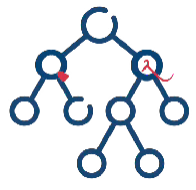
\includegraphics[height=0.9cm]{msca_logo.png}}%
  \end{center}
  \vspace{0.45cm}
  \begin{center}
    \begin{minipage}{0.1\textwidth}\centering
      \href{https://quantlet.com}{
\includegraphics[height=0.9cm]{ql_logo.png}}\end{minipage}%
    \begin{minipage}{0.78\textwidth}\centering
      {\Large\bfseries\usebeamercolor[fg]{title}\inserttitle}\par\vspace{0.25cm}
      {\large\usebeamercolor[fg]{title}\insertsubtitle}\end{minipage}%
    \begin{minipage}{0.1\textwidth}\centering
      \href{https://quantinar.com}{
\includegraphics[height=0.9cm]{qr_logo.png}}\end{minipage}
  \end{center}
  \vfill
  \hspace{0.4cm}{\bfseries\insertauthor}\par\vspace{0.12cm}
  \hspace{0.4cm}\begin{minipage}[t]{0.92\textwidth}\raggedright\footnotesize\insertinstitute\end{minipage}
  \par\vspace{0.4cm}}

% ---------------------------------------------------------------- lecture metadata
\newcommand{\nnshort}{}
\newcommand{\nnnb}{notebooks}
\newcommand{\nnrepo}{https://github.com/danpele/NEURAL_BIZ/tree/main}
% language-dependent labels (English default; \nnromanian switches to Romanian, call it before \nnlecture)
\newcommand{\txtcourse}{Neural Networks and Deep Learning}
\newcommand{\txtlecture}{Lecture}
\newcommand{\txtoutline}{Outline}
\newcommand{\txtintuition}{In one sentence:}
\newcommand{\txtjob}{In practice:}
\newcommand{\txttry}{Experiment yourself:}
\newcommand{\txtwhere}{where}
\newcommand{\txtsim}{SIMULATED DATA (teaching illustration)}
\newcommand{\txtnbsuffix}{}
\newcommand{\txtinstitute}{Bucharest University of Economic Studies (ASE), Department of Statistics and Econometrics\\
    Romanian Academy, Institute for Economic Forecasting (IPE)\\
    IDA Institute Digital Assets \textbullet\ AI4EFin \textbullet\ MSCA Digital Finance}
\newcommand{\nnromanian}{%
  \renewcommand{\txtcourse}{Rețele neuronale și deep learning}%
  \renewcommand{\txtlecture}{Cursul}%
  \renewcommand{\txtoutline}{Cuprins}%
  \renewcommand{\txtintuition}{Pe scurt:}%
  \renewcommand{\txtjob}{În practică:}%
  \renewcommand{\txttry}{Exercițiu practic:}%
  \renewcommand{\txtwhere}{unde}%
  \renewcommand{\txtsim}{DATE SIMULATE (doar pentru ilustrare)}%
  \renewcommand{\txtnbsuffix}{\string_ro}%
  \renewcommand{\txtinstitute}{Academia de Studii Economice din București (ASE), Departamentul de Statistică și Econometrie\\
    Academia Română, Institutul de Prognoză Economică (IPE)\\
    IDA Institute Digital Assets \textbullet\ AI4EFin \textbullet\ MSCA Digital Finance}}
\newcommand{\nnlecture}[2]{%
  \renewcommand{\nnshort}{\txtlecture\ #1}%
  \renewcommand{\nnnb}{notebooks/L#1\string_notebook\txtnbsuffix.ipynb}%
  \title[NN]{\txtcourse}%
  \subtitle{\txtlecture\ #1: #2}%
  \author{Prof.\ dr.\ Daniel Traian PELE}%
  \institute{\txtinstitute}%
  \date{}}

% ---------------------------------------------------------------- teaching blocks (one message per frame)
% \intuition{one plain sentence}  ->  formula with every symbol defined  ->  real-data example  ->  \manager{one line}
\newcommand{\intuition}[1]{\begin{itemize}\item {\color{MainBlue}\textbf{\txtintuition}}~#1\end{itemize}\vspace{0.6mm}}
\newcommand{\manager}[1]{\colorbox{Forest!10}{\parbox{\dimexpr\linewidth-2\fboxsep\relax}{\footnotesize
  \begin{itemize}\setlength{\itemsep}{0pt}\item \textbf{\color{Forest}\txtjob}~#1\end{itemize}}}}
% Experiment yourself: pointer to the matching notebook section
\newcommand{\tryit}[1]{{\scriptsize\href{\nnrepo/\nnnb}{%
  \raisebox{-0.15em}{
\includegraphics[height=0.85em]{ql_logo.png}}\,\textbf{\txttry}~\color{MainBlue}#1}}}
% bottom row: manager line (left) + experiment pointer (right), pinned to the bottom of the frame
\newcommand{\bottomrow}[2]{\par\vfill\noindent\begin{minipage}[b]{0.72\linewidth}#1\end{minipage}\hfill
  \begin{minipage}[b]{0.26\linewidth}\raggedleft #2\end{minipage}\par\vspace{0.5mm}}
\newcommand{\where}[1]{{\footnotesize\textbf{\txtwhere}~#1\par}}

% ---------------------------------------------------------------- helpers
% chart source line under a figure: \chartsource{Source ...; period ...}
\newcommand{\chartsource}[1]{\par\vspace{1pt}{\scriptsize\color{FooterGray}#1\par}}
% link to code: \quantlet{label}{path inside the repo}
\newcommand{\quantlet}[2]{\par\vspace{1pt}\hfill\href{\nnrepo/#2}{%
  \raisebox{-0.15em}{
\includegraphics[height=0.75em]{ql_logo.png}}\textcolor{MainBlue}{\scriptsize\ #1}}}
% inline Quantlet link for the bottom-right corner of a frame: \qlink{label}{path inside the repo}
\newcommand{\qlink}[2]{{\scriptsize\href{\nnrepo/#2}{\raisebox{-0.15em}{
\includegraphics[height=0.85em]{ql_logo.png}}\,\textcolor{MainBlue}{#1}}}}
\newcommand{\simlabel}{\colorbox{Crimson!12}{\scriptsize\bfseries\color{Crimson}\txtsim}}
\newcommand{\E}{\mathbb{E}}
\newcommand{\Var}{\operatorname{Var}}
\newcommand{\Cov}{\operatorname{Cov}}
\newcommand{\Corr}{\operatorname{Corr}}
\newcommand{\asinh}{\operatorname{asinh}}
\newcommand{\iid}{\overset{\text{i.i.d.}}{\sim}}
\newcommand{\EUR}{EUR}
% deep-learning notation (Bishop & Bishop, 2024): vectors bold lower case, matrices bold upper case
\newcommand{\R}{\mathbb{R}}
\newcommand{\vx}{\mathbf{x}}
\newcommand{\vy}{\mathbf{y}}
\newcommand{\vz}{\mathbf{z}}
\newcommand{\vh}{\mathbf{h}}
\newcommand{\vw}{\mathbf{w}}
\newcommand{\vb}{\mathbf{b}}
\newcommand{\mW}{\mathbf{W}}
\newcommand{\mX}{\mathbf{X}}
\newcommand{\btheta}{\boldsymbol{\theta}}
\newcommand{\loss}{\mathcal{L}}
\newcommand{\dataset}{\mathcal{D}}
\DeclareMathOperator*{\argmin}{arg\,min}
\DeclareMathOperator*{\argmax}{arg\,max}
\DeclareMathOperator{\softmax}{softmax}
\DeclareMathOperator{\ReLU}{ReLU}
\DeclareMathOperator{\sigm}{\sigma}

%   \nnlecture{k}{Lecture title}
% Logos live in lectures/common/logos/, charts in lectures/Lk/charts/.
% Do NOT add \hfuzz / \vfuzz / \hbadness here: overfull boxes must be fixed, not hidden.
% =============================================================================

\usetheme{default}
\setbeamersize{text margin left=7mm, text margin right=7mm}

% ---------------------------------------------------------------- packages
\usepackage[utf8]{inputenc}
\usepackage[T1]{fontenc}
\usepackage{lmodern}
\usepackage{amsmath, amssymb}
\usepackage{mathtools}
\usepackage{bm}
\usepackage{tikz}
\usetikzlibrary{arrows.meta, positioning, calc, shapes.misc}
\usepackage{booktabs}
\usepackage{array}
\usepackage{graphicx}
\usepackage{colortbl}
\usepackage{xcolor}
\usepackage{multicol}
\hypersetup{colorlinks=true, linkcolor=MainBlue, urlcolor=MainBlue, citecolor=MainBlue}
\graphicspath{{../common/logos/}}   % charts are included with their language folder: charts/en/, charts/ro/

% ---------------------------------------------------------------- colours
\definecolor{MainBlue}{RGB}{26, 58, 110}
\definecolor{IDAred}{RGB}{205, 0, 0}
\definecolor{DarkGray}{RGB}{51, 51, 51}
\definecolor{FooterGray}{RGB}{100, 100, 100}
\definecolor{BlockGray}{RGB}{236, 238, 242}
\definecolor{KeynoteGray}{RGB}{218, 218, 218}
\definecolor{Crimson}{RGB}{190, 40, 50}
\definecolor{Forest}{RGB}{30, 110, 50}
\definecolor{Bitter}{RGB}{214, 150, 20}
% chart palette (same hex values and order as lectures/common/nn_plot.py SERIES)
\definecolor{Ser1}{HTML}{2A78D6}
\definecolor{Ser2}{HTML}{EB6834}
\definecolor{Ser3}{HTML}{1BAF7A}
\definecolor{Ser4}{HTML}{EDA100}
\definecolor{Ser5}{HTML}{E87BA4}
\definecolor{Ser6}{HTML}{008300}
\definecolor{Ser7}{HTML}{6250D6}
\definecolor{Ser8}{HTML}{E34948}

\setbeamertemplate{background}{%
  \begin{tikzpicture}[remember picture, overlay]
    \shade[shading=axis, shading angle=315, top color=white, bottom color=KeynoteGray]
      (current page.south west) rectangle (current page.north east);
  \end{tikzpicture}}
\setbeamercolor{background canvas}{bg=}
\setbeamercolor{structure}{fg=MainBlue}
\setbeamercolor{normal text}{fg=DarkGray}
\setbeamercolor{title}{fg=IDAred}
\setbeamercolor{frametitle}{fg=IDAred, bg=}
\setbeamercolor{block title}{bg=MainBlue, fg=white}
\setbeamercolor{block body}{bg=BlockGray, fg=DarkGray}
\setbeamercolor{block title alerted}{bg=Crimson, fg=white}
\setbeamercolor{block body alerted}{bg=Crimson!7, fg=DarkGray}
\setbeamercolor{block title example}{bg=Forest, fg=white}
\setbeamercolor{block body example}{bg=Forest!7, fg=DarkGray}
\setbeamercolor{item}{fg=MainBlue}
\setbeamerfont{frametitle}{size=\large, series=\bfseries}
\setbeamerfont{block title}{size=\small, series=\bfseries}
\setbeamertemplate{blocks}[rounded][shadow=false]
\setbeamertemplate{itemize item}{\color{MainBlue}$\boxdot$}
\setbeamertemplate{itemize subitem}{\color{MainBlue}\scriptsize$\blacktriangleright$}
% compact two-level lists: level 1 = main point, level 2 = details (no text outside bullets)
\setbeamerfont{itemize/enumerate subbody}{size=\footnotesize}
\setlength{\leftmargini}{1.1em}
\setlength{\leftmarginii}{1.1em}
\setbeamertemplate{itemize/enumerate body begin}{\setlength{\topsep}{0pt}\setlength{\partopsep}{0pt}\setlength{\parskip}{0pt}}
\setbeamertemplate{itemize/enumerate subbody begin}{\setlength{\topsep}{0pt}\setlength{\partopsep}{0pt}\setlength{\itemsep}{0pt}\vspace{-0.4ex}}

\setbeamertemplate{enumerate item}{\color{MainBlue}\insertenumlabel.}
\setlength{\leftmargini}{1.3em}
\setlength{\leftmarginii}{1.2em}
\setbeamertemplate{navigation symbols}{}
\setbeamertemplate{section in toc}{\color{MainBlue}$\blacktriangleright$~\inserttocsection}
\setbeamertemplate{caption}{\raggedright\insertcaption\par}
% frame subtitle = precise citation line under the claim title (Weron style)
\setbeamerfont{framesubtitle}{size=\footnotesize}
\setbeamercolor{framesubtitle}{fg=FooterGray}
% outline that reappears at every section with the current section highlighted
\setbeamertemplate{section in toc shaded}[default][35]
\setbeamertemplate{subsection in toc shaded}[default][35]
\setbeamertemplate{subsection in toc}{\leavevmode\leftskip=2.2em\color{DarkGray}\small\inserttocsubsection\par}
\AtBeginSection[]{{\begin{frame}{\txtoutline}\vspace{2mm}\small
  \tableofcontents[currentsection,hideothersubsections]\end{frame}}}

% ---------------------------------------------------------------- head and foot
\setbeamertemplate{headline}{%
  \vskip10pt%
  \hbox to \paperwidth{\hskip0.5cm%
    {\small\color{FooterGray}\renewcommand{\hyperlink}[2]{##2}\insertsectionhead}%
    \hfill\textcolor{FooterGray}{\small\insertframenumber}\hskip0.5cm}%
  \vskip4pt{\color{FooterGray}\hrule height 0.4pt}}
% footer as in the other courses (MFM, SFM): course name on the left, small sparkline on the right
\setbeamertemplate{footline}{%
  {\color{FooterGray}\hrule height 0.4pt}\vskip4pt%
  \hbox to \paperwidth{\hskip0.5cm%
    \textcolor{FooterGray}{\small\txtcourse}%
    \hfill\raisebox{-0.1em}{\begin{tikzpicture}[x=0.08em, y=0.08em, line width=0.4pt]
      \draw[FooterGray] (0,3) -- (1,4) -- (2,3.5) -- (3,5) -- (4,4) -- (5,6) -- (6,5.5) -- (7,4) -- (8,5) -- (9,7) -- (10,6) -- (11,5) -- (12,6.5) -- (13,8) -- (14,7) -- (15,6) -- (16,7.5) -- (17,9) -- (18,8) -- (19,7) -- (20,8.5) -- (21,10) -- (22,9) -- (23,8) -- (24,9.5);
    \end{tikzpicture}}\hskip0.5cm}%
  \vskip6pt}

% ---------------------------------------------------------------- title page
\defbeamertemplate*{title page}{nn}[1][]{%
  \vspace{0.15cm}
  \begin{center}
    \href{https://www.ase.ro}{
\includegraphics[height=0.9cm]{ase_logo.png}}\hspace{0.3cm}%
    \href{https://ipe.ro/new}{
\includegraphics[height=0.9cm]{acad_logo.png}}\hspace{0.3cm}%
    \href{https://theida.net}{
\includegraphics[height=0.9cm]{ida_logo.png}}\hspace{0.3cm}%
    \href{https://blockchain-research-center.com}{
\includegraphics[height=0.9cm]{brc_logo.png}}\hspace{0.3cm}%
    \href{https://www.ai4efin.ase.ro}{
\includegraphics[height=0.9cm]{ai4efin_logo.png}}\hspace{0.3cm}%
    \href{https://www.digital-finance-msca.com}{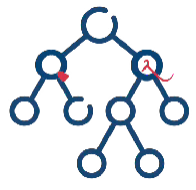
\includegraphics[height=0.9cm]{msca_logo.png}}%
  \end{center}
  \vspace{0.45cm}
  \begin{center}
    \begin{minipage}{0.1\textwidth}\centering
      \href{https://quantlet.com}{
\includegraphics[height=0.9cm]{ql_logo.png}}\end{minipage}%
    \begin{minipage}{0.78\textwidth}\centering
      {\Large\bfseries\usebeamercolor[fg]{title}\inserttitle}\par\vspace{0.25cm}
      {\large\usebeamercolor[fg]{title}\insertsubtitle}\end{minipage}%
    \begin{minipage}{0.1\textwidth}\centering
      \href{https://quantinar.com}{
\includegraphics[height=0.9cm]{qr_logo.png}}\end{minipage}
  \end{center}
  \vfill
  \hspace{0.4cm}{\bfseries\insertauthor}\par\vspace{0.12cm}
  \hspace{0.4cm}\begin{minipage}[t]{0.92\textwidth}\raggedright\footnotesize\insertinstitute\end{minipage}
  \par\vspace{0.4cm}}

% ---------------------------------------------------------------- lecture metadata
\newcommand{\nnshort}{}
\newcommand{\nnnb}{notebooks}
\newcommand{\nnrepo}{https://github.com/danpele/NEURAL_BIZ/tree/main}
% language-dependent labels (English default; \nnromanian switches to Romanian, call it before \nnlecture)
\newcommand{\txtcourse}{Neural Networks and Deep Learning}
\newcommand{\txtlecture}{Lecture}
\newcommand{\txtoutline}{Outline}
\newcommand{\txtintuition}{In one sentence:}
\newcommand{\txtjob}{In practice:}
\newcommand{\txttry}{Experiment yourself:}
\newcommand{\txtwhere}{where}
\newcommand{\txtsim}{SIMULATED DATA (teaching illustration)}
\newcommand{\txtnbsuffix}{}
\newcommand{\txtinstitute}{Bucharest University of Economic Studies (ASE), Department of Statistics and Econometrics\\
    Romanian Academy, Institute for Economic Forecasting (IPE)\\
    IDA Institute Digital Assets \textbullet\ AI4EFin \textbullet\ MSCA Digital Finance}
\newcommand{\nnromanian}{%
  \renewcommand{\txtcourse}{Rețele neuronale și deep learning}%
  \renewcommand{\txtlecture}{Cursul}%
  \renewcommand{\txtoutline}{Cuprins}%
  \renewcommand{\txtintuition}{Pe scurt:}%
  \renewcommand{\txtjob}{În practică:}%
  \renewcommand{\txttry}{Exercițiu practic:}%
  \renewcommand{\txtwhere}{unde}%
  \renewcommand{\txtsim}{DATE SIMULATE (doar pentru ilustrare)}%
  \renewcommand{\txtnbsuffix}{\string_ro}%
  \renewcommand{\txtinstitute}{Academia de Studii Economice din București (ASE), Departamentul de Statistică și Econometrie\\
    Academia Română, Institutul de Prognoză Economică (IPE)\\
    IDA Institute Digital Assets \textbullet\ AI4EFin \textbullet\ MSCA Digital Finance}}
\newcommand{\nnlecture}[2]{%
  \renewcommand{\nnshort}{\txtlecture\ #1}%
  \renewcommand{\nnnb}{notebooks/L#1\string_notebook\txtnbsuffix.ipynb}%
  \title[NN]{\txtcourse}%
  \subtitle{\txtlecture\ #1: #2}%
  \author{Prof.\ dr.\ Daniel Traian PELE}%
  \institute{\txtinstitute}%
  \date{}}

% ---------------------------------------------------------------- teaching blocks (one message per frame)
% \intuition{one plain sentence}  ->  formula with every symbol defined  ->  real-data example  ->  \manager{one line}
\newcommand{\intuition}[1]{\begin{itemize}\item {\color{MainBlue}\textbf{\txtintuition}}~#1\end{itemize}\vspace{0.6mm}}
\newcommand{\manager}[1]{\colorbox{Forest!10}{\parbox{\dimexpr\linewidth-2\fboxsep\relax}{\footnotesize
  \begin{itemize}\setlength{\itemsep}{0pt}\item \textbf{\color{Forest}\txtjob}~#1\end{itemize}}}}
% Experiment yourself: pointer to the matching notebook section
\newcommand{\tryit}[1]{{\scriptsize\href{\nnrepo/\nnnb}{%
  \raisebox{-0.15em}{
\includegraphics[height=0.85em]{ql_logo.png}}\,\textbf{\txttry}~\color{MainBlue}#1}}}
% bottom row: manager line (left) + experiment pointer (right), pinned to the bottom of the frame
\newcommand{\bottomrow}[2]{\par\vfill\noindent\begin{minipage}[b]{0.72\linewidth}#1\end{minipage}\hfill
  \begin{minipage}[b]{0.26\linewidth}\raggedleft #2\end{minipage}\par\vspace{0.5mm}}
\newcommand{\where}[1]{{\footnotesize\textbf{\txtwhere}~#1\par}}

% ---------------------------------------------------------------- helpers
% chart source line under a figure: \chartsource{Source ...; period ...}
\newcommand{\chartsource}[1]{\par\vspace{1pt}{\scriptsize\color{FooterGray}#1\par}}
% link to code: \quantlet{label}{path inside the repo}
\newcommand{\quantlet}[2]{\par\vspace{1pt}\hfill\href{\nnrepo/#2}{%
  \raisebox{-0.15em}{
\includegraphics[height=0.75em]{ql_logo.png}}\textcolor{MainBlue}{\scriptsize\ #1}}}
% inline Quantlet link for the bottom-right corner of a frame: \qlink{label}{path inside the repo}
\newcommand{\qlink}[2]{{\scriptsize\href{\nnrepo/#2}{\raisebox{-0.15em}{
\includegraphics[height=0.85em]{ql_logo.png}}\,\textcolor{MainBlue}{#1}}}}
\newcommand{\simlabel}{\colorbox{Crimson!12}{\scriptsize\bfseries\color{Crimson}\txtsim}}
\newcommand{\E}{\mathbb{E}}
\newcommand{\Var}{\operatorname{Var}}
\newcommand{\Cov}{\operatorname{Cov}}
\newcommand{\Corr}{\operatorname{Corr}}
\newcommand{\asinh}{\operatorname{asinh}}
\newcommand{\iid}{\overset{\text{i.i.d.}}{\sim}}
\newcommand{\EUR}{EUR}
% deep-learning notation (Bishop & Bishop, 2024): vectors bold lower case, matrices bold upper case
\newcommand{\R}{\mathbb{R}}
\newcommand{\vx}{\mathbf{x}}
\newcommand{\vy}{\mathbf{y}}
\newcommand{\vz}{\mathbf{z}}
\newcommand{\vh}{\mathbf{h}}
\newcommand{\vw}{\mathbf{w}}
\newcommand{\vb}{\mathbf{b}}
\newcommand{\mW}{\mathbf{W}}
\newcommand{\mX}{\mathbf{X}}
\newcommand{\btheta}{\boldsymbol{\theta}}
\newcommand{\loss}{\mathcal{L}}
\newcommand{\dataset}{\mathcal{D}}
\DeclareMathOperator*{\argmin}{arg\,min}
\DeclareMathOperator*{\argmax}{arg\,max}
\DeclareMathOperator{\softmax}{softmax}
\DeclareMathOperator{\ReLU}{ReLU}
\DeclareMathOperator{\sigm}{\sigma}

%   \nnlecture{k}{Lecture title}
% Logos live in lectures/common/logos/, charts in lectures/Lk/charts/.
% Do NOT add \hfuzz / \vfuzz / \hbadness here: overfull boxes must be fixed, not hidden.
% =============================================================================

\usetheme{default}
\setbeamersize{text margin left=7mm, text margin right=7mm}

% ---------------------------------------------------------------- packages
\usepackage[utf8]{inputenc}
\usepackage[T1]{fontenc}
\usepackage{lmodern}
\usepackage{amsmath, amssymb}
\usepackage{mathtools}
\usepackage{bm}
\usepackage{tikz}
\usetikzlibrary{arrows.meta, positioning, calc, shapes.misc}
\usepackage{booktabs}
\usepackage{array}
\usepackage{graphicx}
\usepackage{colortbl}
\usepackage{xcolor}
\usepackage{multicol}
\hypersetup{colorlinks=true, linkcolor=MainBlue, urlcolor=MainBlue, citecolor=MainBlue}
\graphicspath{{../common/logos/}}   % charts are included with their language folder: charts/en/, charts/ro/

% ---------------------------------------------------------------- colours
\definecolor{MainBlue}{RGB}{26, 58, 110}
\definecolor{IDAred}{RGB}{205, 0, 0}
\definecolor{DarkGray}{RGB}{51, 51, 51}
\definecolor{FooterGray}{RGB}{100, 100, 100}
\definecolor{BlockGray}{RGB}{236, 238, 242}
\definecolor{KeynoteGray}{RGB}{218, 218, 218}
\definecolor{Crimson}{RGB}{190, 40, 50}
\definecolor{Forest}{RGB}{30, 110, 50}
\definecolor{Bitter}{RGB}{214, 150, 20}
% chart palette (same hex values and order as lectures/common/nn_plot.py SERIES)
\definecolor{Ser1}{HTML}{2A78D6}
\definecolor{Ser2}{HTML}{EB6834}
\definecolor{Ser3}{HTML}{1BAF7A}
\definecolor{Ser4}{HTML}{EDA100}
\definecolor{Ser5}{HTML}{E87BA4}
\definecolor{Ser6}{HTML}{008300}
\definecolor{Ser7}{HTML}{6250D6}
\definecolor{Ser8}{HTML}{E34948}

\setbeamertemplate{background}{%
  \begin{tikzpicture}[remember picture, overlay]
    \shade[shading=axis, shading angle=315, top color=white, bottom color=KeynoteGray]
      (current page.south west) rectangle (current page.north east);
  \end{tikzpicture}}
\setbeamercolor{background canvas}{bg=}
\setbeamercolor{structure}{fg=MainBlue}
\setbeamercolor{normal text}{fg=DarkGray}
\setbeamercolor{title}{fg=IDAred}
\setbeamercolor{frametitle}{fg=IDAred, bg=}
\setbeamercolor{block title}{bg=MainBlue, fg=white}
\setbeamercolor{block body}{bg=BlockGray, fg=DarkGray}
\setbeamercolor{block title alerted}{bg=Crimson, fg=white}
\setbeamercolor{block body alerted}{bg=Crimson!7, fg=DarkGray}
\setbeamercolor{block title example}{bg=Forest, fg=white}
\setbeamercolor{block body example}{bg=Forest!7, fg=DarkGray}
\setbeamercolor{item}{fg=MainBlue}
\setbeamerfont{frametitle}{size=\large, series=\bfseries}
\setbeamerfont{block title}{size=\small, series=\bfseries}
\setbeamertemplate{blocks}[rounded][shadow=false]
\setbeamertemplate{itemize item}{\color{MainBlue}$\boxdot$}
\setbeamertemplate{itemize subitem}{\color{MainBlue}\scriptsize$\blacktriangleright$}
% compact two-level lists: level 1 = main point, level 2 = details (no text outside bullets)
\setbeamerfont{itemize/enumerate subbody}{size=\footnotesize}
\setlength{\leftmargini}{1.1em}
\setlength{\leftmarginii}{1.1em}
\setbeamertemplate{itemize/enumerate body begin}{\setlength{\topsep}{0pt}\setlength{\partopsep}{0pt}\setlength{\parskip}{0pt}}
\setbeamertemplate{itemize/enumerate subbody begin}{\setlength{\topsep}{0pt}\setlength{\partopsep}{0pt}\setlength{\itemsep}{0pt}\vspace{-0.4ex}}

\setbeamertemplate{enumerate item}{\color{MainBlue}\insertenumlabel.}
\setlength{\leftmargini}{1.3em}
\setlength{\leftmarginii}{1.2em}
\setbeamertemplate{navigation symbols}{}
\setbeamertemplate{section in toc}{\color{MainBlue}$\blacktriangleright$~\inserttocsection}
\setbeamertemplate{caption}{\raggedright\insertcaption\par}
% frame subtitle = precise citation line under the claim title (Weron style)
\setbeamerfont{framesubtitle}{size=\footnotesize}
\setbeamercolor{framesubtitle}{fg=FooterGray}
% outline that reappears at every section with the current section highlighted
\setbeamertemplate{section in toc shaded}[default][35]
\setbeamertemplate{subsection in toc shaded}[default][35]
\setbeamertemplate{subsection in toc}{\leavevmode\leftskip=2.2em\color{DarkGray}\small\inserttocsubsection\par}
\AtBeginSection[]{{\begin{frame}{\txtoutline}\vspace{2mm}\small
  \tableofcontents[currentsection,hideothersubsections]\end{frame}}}

% ---------------------------------------------------------------- head and foot
\setbeamertemplate{headline}{%
  \vskip10pt%
  \hbox to \paperwidth{\hskip0.5cm%
    {\small\color{FooterGray}\renewcommand{\hyperlink}[2]{##2}\insertsectionhead}%
    \hfill\textcolor{FooterGray}{\small\insertframenumber}\hskip0.5cm}%
  \vskip4pt{\color{FooterGray}\hrule height 0.4pt}}
% footer as in the other courses (MFM, SFM): course name on the left, small sparkline on the right
\setbeamertemplate{footline}{%
  {\color{FooterGray}\hrule height 0.4pt}\vskip4pt%
  \hbox to \paperwidth{\hskip0.5cm%
    \textcolor{FooterGray}{\small\txtcourse}%
    \hfill\raisebox{-0.1em}{\begin{tikzpicture}[x=0.08em, y=0.08em, line width=0.4pt]
      \draw[FooterGray] (0,3) -- (1,4) -- (2,3.5) -- (3,5) -- (4,4) -- (5,6) -- (6,5.5) -- (7,4) -- (8,5) -- (9,7) -- (10,6) -- (11,5) -- (12,6.5) -- (13,8) -- (14,7) -- (15,6) -- (16,7.5) -- (17,9) -- (18,8) -- (19,7) -- (20,8.5) -- (21,10) -- (22,9) -- (23,8) -- (24,9.5);
    \end{tikzpicture}}\hskip0.5cm}%
  \vskip6pt}

% ---------------------------------------------------------------- title page
\defbeamertemplate*{title page}{nn}[1][]{%
  \vspace{0.15cm}
  \begin{center}
    \href{https://www.ase.ro}{
\includegraphics[height=0.9cm]{ase_logo.png}}\hspace{0.3cm}%
    \href{https://ipe.ro/new}{
\includegraphics[height=0.9cm]{acad_logo.png}}\hspace{0.3cm}%
    \href{https://theida.net}{
\includegraphics[height=0.9cm]{ida_logo.png}}\hspace{0.3cm}%
    \href{https://blockchain-research-center.com}{
\includegraphics[height=0.9cm]{brc_logo.png}}\hspace{0.3cm}%
    \href{https://www.ai4efin.ase.ro}{
\includegraphics[height=0.9cm]{ai4efin_logo.png}}\hspace{0.3cm}%
    \href{https://www.digital-finance-msca.com}{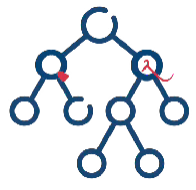
\includegraphics[height=0.9cm]{msca_logo.png}}%
  \end{center}
  \vspace{0.45cm}
  \begin{center}
    \begin{minipage}{0.1\textwidth}\centering
      \href{https://quantlet.com}{
\includegraphics[height=0.9cm]{ql_logo.png}}\end{minipage}%
    \begin{minipage}{0.78\textwidth}\centering
      {\Large\bfseries\usebeamercolor[fg]{title}\inserttitle}\par\vspace{0.25cm}
      {\large\usebeamercolor[fg]{title}\insertsubtitle}\end{minipage}%
    \begin{minipage}{0.1\textwidth}\centering
      \href{https://quantinar.com}{
\includegraphics[height=0.9cm]{qr_logo.png}}\end{minipage}
  \end{center}
  \vfill
  \hspace{0.4cm}{\bfseries\insertauthor}\par\vspace{0.12cm}
  \hspace{0.4cm}\begin{minipage}[t]{0.92\textwidth}\raggedright\footnotesize\insertinstitute\end{minipage}
  \par\vspace{0.4cm}}

% ---------------------------------------------------------------- lecture metadata
\newcommand{\nnshort}{}
\newcommand{\nnnb}{notebooks}
\newcommand{\nnrepo}{https://github.com/danpele/NEURAL_BIZ/tree/main}
% language-dependent labels (English default; \nnromanian switches to Romanian, call it before \nnlecture)
\newcommand{\txtcourse}{Neural Networks and Deep Learning}
\newcommand{\txtlecture}{Lecture}
\newcommand{\txtoutline}{Outline}
\newcommand{\txtintuition}{In one sentence:}
\newcommand{\txtjob}{In practice:}
\newcommand{\txttry}{Experiment yourself:}
\newcommand{\txtwhere}{where}
\newcommand{\txtsim}{SIMULATED DATA (teaching illustration)}
\newcommand{\txtnbsuffix}{}
\newcommand{\txtinstitute}{Bucharest University of Economic Studies (ASE), Department of Statistics and Econometrics\\
    Romanian Academy, Institute for Economic Forecasting (IPE)\\
    IDA Institute Digital Assets \textbullet\ AI4EFin \textbullet\ MSCA Digital Finance}
\newcommand{\nnromanian}{%
  \renewcommand{\txtcourse}{Rețele neuronale și deep learning}%
  \renewcommand{\txtlecture}{Cursul}%
  \renewcommand{\txtoutline}{Cuprins}%
  \renewcommand{\txtintuition}{Pe scurt:}%
  \renewcommand{\txtjob}{În practică:}%
  \renewcommand{\txttry}{Exercițiu practic:}%
  \renewcommand{\txtwhere}{unde}%
  \renewcommand{\txtsim}{DATE SIMULATE (doar pentru ilustrare)}%
  \renewcommand{\txtnbsuffix}{\string_ro}%
  \renewcommand{\txtinstitute}{Academia de Studii Economice din București (ASE), Departamentul de Statistică și Econometrie\\
    Academia Română, Institutul de Prognoză Economică (IPE)\\
    IDA Institute Digital Assets \textbullet\ AI4EFin \textbullet\ MSCA Digital Finance}}
\newcommand{\nnlecture}[2]{%
  \renewcommand{\nnshort}{\txtlecture\ #1}%
  \renewcommand{\nnnb}{notebooks/L#1\string_notebook\txtnbsuffix.ipynb}%
  \title[NN]{\txtcourse}%
  \subtitle{\txtlecture\ #1: #2}%
  \author{Prof.\ dr.\ Daniel Traian PELE}%
  \institute{\txtinstitute}%
  \date{}}

% ---------------------------------------------------------------- teaching blocks (one message per frame)
% \intuition{one plain sentence}  ->  formula with every symbol defined  ->  real-data example  ->  \manager{one line}
\newcommand{\intuition}[1]{\begin{itemize}\item {\color{MainBlue}\textbf{\txtintuition}}~#1\end{itemize}\vspace{0.6mm}}
\newcommand{\manager}[1]{\colorbox{Forest!10}{\parbox{\dimexpr\linewidth-2\fboxsep\relax}{\footnotesize
  \begin{itemize}\setlength{\itemsep}{0pt}\item \textbf{\color{Forest}\txtjob}~#1\end{itemize}}}}
% Experiment yourself: pointer to the matching notebook section
\newcommand{\tryit}[1]{{\scriptsize\href{\nnrepo/\nnnb}{%
  \raisebox{-0.15em}{
\includegraphics[height=0.85em]{ql_logo.png}}\,\textbf{\txttry}~\color{MainBlue}#1}}}
% bottom row: manager line (left) + experiment pointer (right), pinned to the bottom of the frame
\newcommand{\bottomrow}[2]{\par\vfill\noindent\begin{minipage}[b]{0.72\linewidth}#1\end{minipage}\hfill
  \begin{minipage}[b]{0.26\linewidth}\raggedleft #2\end{minipage}\par\vspace{0.5mm}}
\newcommand{\where}[1]{{\footnotesize\textbf{\txtwhere}~#1\par}}

% ---------------------------------------------------------------- helpers
% chart source line under a figure: \chartsource{Source ...; period ...}
\newcommand{\chartsource}[1]{\par\vspace{1pt}{\scriptsize\color{FooterGray}#1\par}}
% link to code: \quantlet{label}{path inside the repo}
\newcommand{\quantlet}[2]{\par\vspace{1pt}\hfill\href{\nnrepo/#2}{%
  \raisebox{-0.15em}{
\includegraphics[height=0.75em]{ql_logo.png}}\textcolor{MainBlue}{\scriptsize\ #1}}}
% inline Quantlet link for the bottom-right corner of a frame: \qlink{label}{path inside the repo}
\newcommand{\qlink}[2]{{\scriptsize\href{\nnrepo/#2}{\raisebox{-0.15em}{
\includegraphics[height=0.85em]{ql_logo.png}}\,\textcolor{MainBlue}{#1}}}}
\newcommand{\simlabel}{\colorbox{Crimson!12}{\scriptsize\bfseries\color{Crimson}\txtsim}}
\newcommand{\E}{\mathbb{E}}
\newcommand{\Var}{\operatorname{Var}}
\newcommand{\Cov}{\operatorname{Cov}}
\newcommand{\Corr}{\operatorname{Corr}}
\newcommand{\asinh}{\operatorname{asinh}}
\newcommand{\iid}{\overset{\text{i.i.d.}}{\sim}}
\newcommand{\EUR}{EUR}
% deep-learning notation (Bishop & Bishop, 2024): vectors bold lower case, matrices bold upper case
\newcommand{\R}{\mathbb{R}}
\newcommand{\vx}{\mathbf{x}}
\newcommand{\vy}{\mathbf{y}}
\newcommand{\vz}{\mathbf{z}}
\newcommand{\vh}{\mathbf{h}}
\newcommand{\vw}{\mathbf{w}}
\newcommand{\vb}{\mathbf{b}}
\newcommand{\mW}{\mathbf{W}}
\newcommand{\mX}{\mathbf{X}}
\newcommand{\btheta}{\boldsymbol{\theta}}
\newcommand{\loss}{\mathcal{L}}
\newcommand{\dataset}{\mathcal{D}}
\DeclareMathOperator*{\argmin}{arg\,min}
\DeclareMathOperator*{\argmax}{arg\,max}
\DeclareMathOperator{\softmax}{softmax}
\DeclareMathOperator{\ReLU}{ReLU}
\DeclareMathOperator{\sigm}{\sigma}

\nnlecture{6}{NLP foundations: text representation and word embeddings}
\begin{document}
{\setbeamertemplate{headline}{}\setbeamertemplate{footline}{}
\begin{frame}\titlepage\end{frame}}
% END-FRONT-MATTER

\begin{frame}{Learning objectives}
\small
\begin{itemize}\setlength{\itemsep}{4pt}
  \item Turn financial text into numbers for natural language processing (NLP): tokens, vocabulary, bag of words and term frequency--inverse document frequency (TF-IDF).
  \item Write the objectives of word2vec and GloVe and train both on a real corpus of central-bank speeches.
  \item Build sentence classifiers from sparse and dense representations, with honest benchmarks and tests.
  \item Measure financial sentiment and topics on news and tweets, and know when a linear model is enough.
\end{itemize}
\end{frame}

% BEGIN-ABBR

\begin{frame}{Abbreviations}
\small
\vspace{-1mm}\begin{columns}[T,onlytextwidth]
\begin{column}{0.49\textwidth}{\scriptsize\renewcommand{\arraystretch}{0.96}\begin{tabular}{@{}>{\bfseries}l@{\ \ }p{0.74\linewidth}@{}}AI & artificial intelligence\\
ASE & Bucharest University of Economic Studies\\
BERT & bidirectional encoder representations from transformers\\
BoW & bag of words\\
CBOW & continuous bag of words (word2vec variant)\\
CPU & central processing unit\\
ECB & European Central Bank\\
ES & expected shortfall\\
ESG & environmental, social and governance\\
FinBERT & BERT model adapted to financial text\\
IPE & Institute for Economic Forecasting, Romanian Academy\\\end{tabular}}\end{column}
\begin{column}{0.49\textwidth}{\scriptsize\renewcommand{\arraystretch}{0.96}\begin{tabular}{@{}>{\bfseries}l@{\ \ }p{0.74\linewidth}@{}}LLM & large language model\\
MLP & multilayer perceptron\\
NLP & natural language processing\\
OOV & out of vocabulary\\
PCA & principal component analysis\\
PMI & pointwise mutual information\\
SGNS & skip-gram with negative sampling\\
SVD & singular value decomposition\\
TF-IDF & term frequency--inverse document frequency\\
VaR & value-at-risk\\\end{tabular}}\end{column}
\end{columns}
\end{frame}

% END-ABBR

\begin{frame}{Real data only: three text collections}
\footnotesize
{\footnotesize\renewcommand{\arraystretch}{1.05}\setlength{\tabcolsep}{4pt}
\begin{tabular}{@{}p{0.23\textwidth}p{0.33\textwidth}p{0.17\textwidth}p{0.18\textwidth}@{}}\toprule
Corpus & Content & Size & Use here \\ \midrule
Financial PhraseBank & sentences of financial news on Finnish listed companies, labelled positive / neutral / negative by 5--8 annotators & 4\,838 sentences & sentiment \\
Twitter financial news & finance tweets: bearish / bullish / neutral, and 20 topics & 9\,543 + 2\,388 (sentiment), 16\,990 + 4\,117 (topic) & sentiment, topics \\
European Central Bank (ECB) speeches & full texts of the Executive Board and Supervisory Board & 400 speeches, 1\,289\,896 tokens & our own embeddings \\
\bottomrule\end{tabular}}
\par\vspace{0.5mm}{\scriptsize \begin{itemize}\setlength{\itemsep}{0pt}
  \item Speeches from 8 Jan 2022 to 30 Oct 2026; PhraseBank by Malo et al. (2014); tweets as published on Hugging Face (train and validation splits).
  \item Every model is trained on the central processing unit (CPU) of a laptop with seed 20261108; test sets are used once.
\end{itemize}}
\par\vfill\noindent{\scriptsize\color{FooterGray}(data/SOURCES.md)}\par\vspace{0.5mm}
\end{frame}


\section{Text as data}

\begin{frame}{From a sentence to tokens}
\footnotesize
\begin{itemize}\setlength{\itemsep}{4pt}
  \item \textbf{A real PhraseBank sentence}
    \begin{itemize}\setlength{\itemsep}{0pt}
      \item ``Finnish Aktia Group 's operating profit rose to EUR 17.5 mn in the first quarter of 2010 from EUR 8.2 mn in the first quarter of 2009 .''
      \item Label given by the annotators: \textbf{positive}
    \end{itemize}
  \item \textbf{Our tokeniser}
    \begin{itemize}\setlength{\itemsep}{0pt}
      \item Lower case, words and numbers; every number becomes \texttt{\textless{}num\textgreater{}}; links and @-mentions removed
      \item First tokens: \texttt{finnish aktia group s operating profit rose to eur \textless{}num\textgreater{} mn in the first} (27 in total)
    \end{itemize}
  \item \textbf{Choices that change results}
    \begin{itemize}\setlength{\itemsep}{0pt}
      \item Lower-casing merges ``Bank'' and ``bank''; stemming merges ``rose'', ``rising''
      \item Removing stop words deletes ``not'', ``down'', ``up'': harmful for sentiment
    \end{itemize}
\end{itemize}
\par\vfill\manager{write the preprocessing down and keep it identical in training and production
    \begin{itemize}\setlength{\itemsep}{0pt}
      \item A different tokeniser is a different model.
    \end{itemize}}\par\vspace{0.5mm}
\par\vfill\noindent{\scriptsize\color{FooterGray}(Malo et al., 2014)}\hfill\tryit{\S1}\par\vspace{0.5mm}
\end{frame}

\begin{frame}{Few words are frequent, most are rare: Zipf's law}
\small
\intuition{in 400 speeches of the European Central Bank, frequency falls as a power of rank.}
\vspace{-1mm}\[ f(r)\approx C\,r^{-a}\quad\Longleftrightarrow\quad\ln f(r)=\ln C-a\ln r \]\vspace{-2mm}
\begin{center}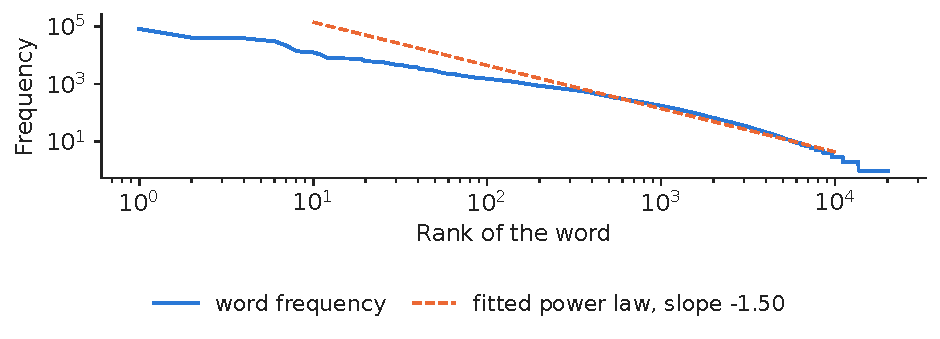
\includegraphics[width=\textwidth,height=0.360\textheight,keepaspectratio]{charts/en/zipf.pdf}\end{center}\vspace{-3mm}
\chartsource{Source: European Central Bank, speeches dataset. Data: 8 Jan 2022 to 30 Oct 2026, 400 speeches.}
\vspace{0.5mm}
\begin{itemize}\setlength{\itemsep}{0pt}
  \item 1\,289\,896 tokens, 20\,130 distinct words
    \begin{itemize}\setlength{\itemsep}{0pt}
      \item Estimated slope \ensuremath{-}1.498 (ranks 10 to 10,000)
      \item The 10 most frequent words make 25.0\,\% of all tokens.
    \end{itemize}
  \item 32.5\,\% of the distinct words occur once: no model can learn them from this corpus alone.
\end{itemize}
\par\vfill\noindent{\scriptsize\color{FooterGray}(Zipf, 1949; own computation)}\hfill\qlink{NN\_L6\_zipf}{Quantlets/L6/NN_L6_zipf}\par\vspace{0.5mm}
\end{frame}


\section{Sparse representations: bag of words and TF-IDF}

\begin{frame}{Bag of words: a document is a vector of counts}
\footnotesize
\intuition{ignore the order, keep how many times each vocabulary word occurs.}
\begin{columns}[T,onlytextwidth]
\begin{column}{0.53\textwidth}
\[ \mathbf x_i=(c_{i1},\dots,c_{iV})^{\top} \]\vspace{-2mm}\[ c_{ij}=\#\{\text{occurrences of word } j \text{ in document } i\} \]{\footnotesize\begin{itemize}\setlength{\itemsep}{0pt}
  \item \textbf{\txtwhere}
    \begin{itemize}\setlength{\itemsep}{0pt}
      \item $V$ vocabulary size (words seen at least twice in the training part)
      \item The document-term matrix $\mathbf C\in\mathbb N^{n\times V}$ is almost all zeros
    \end{itemize}
\end{itemize}\par}
\end{column}
\begin{column}{0.44\textwidth}
\begin{itemize}\setlength{\itemsep}{2pt}
  \item Bag of words (BoW) + multinomial logistic regression is the standard text baseline.
  \item $n$-grams add local order: ``profit rose'' and ``profit fell'' become features.
  \item Vocabulary is fitted on the training sentences only.
\end{itemize}
\end{column}
\end{columns}
\par\vfill\manager{BoW models are fast, cheap and explainable word by word: auditors like them.}\par\vspace{0.5mm}
\par\vfill\noindent{\scriptsize\color{FooterGray}(Salton \& Buckley, 1988)}\par\vspace{0.5mm}
\end{frame}

\begin{frame}{TF-IDF: down-weight words that appear everywhere}
\footnotesize
\intuition{a word is informative if it is frequent in this document and rare in the others.}
\begin{columns}[T,onlytextwidth]
\begin{column}{0.53\textwidth}
\[ w_{ij}=\underbrace{(1+\ln c_{ij})}_{\text{tf}}\cdot\underbrace{\Big(\ln\frac{1+n}{1+n_j}+1\Big)}_{\text{idf}},\qquad \tilde{\mathbf x}_i=\frac{\mathbf w_i}{\|\mathbf w_i\|_2} \]{\footnotesize\begin{itemize}\setlength{\itemsep}{0pt}
  \item \textbf{\txtwhere}
    \begin{itemize}\setlength{\itemsep}{0pt}
      \item $c_{ij}>0$ count of term $j$ in document $i$ ($w_{ij}=0$ if $c_{ij}=0$)
      \item $n$ documents
      \item $n_j$ documents containing $j$
      \item Sublinear tf and smoothed idf, as in scikit-learn
    \end{itemize}
\end{itemize}\par}
\end{column}
\begin{column}{0.44\textwidth}
\begin{itemize}\setlength{\itemsep}{2pt}
  \item Term frequency--inverse document frequency (TF-IDF) on unigrams and bigrams, then logistic regression with balanced class weights.
  \item Words like ``the'', ``company'', \texttt{\textless{}num\textgreater{}} get a low idf
    \begin{itemize}\setlength{\itemsep}{0pt}
      \item ``plunged'' a high one.
    \end{itemize}
  \item The $\ell_2$ normalisation makes long and short sentences comparable.
\end{itemize}
\end{column}
\end{columns}
\par\vfill\manager{TF-IDF + logistic regression is the model any NLP vendor must beat on your own documents.}\par\vspace{0.5mm}
\par\vfill\noindent{\scriptsize\color{FooterGray}(Salton \& Buckley, 1988)}\par\vspace{0.5mm}
\end{frame}

\begin{frame}{The linear model learns a finance sentiment dictionary}
\small
\intuition{the difference between the positive and negative coefficients of each word, logistic regression on BoW, PhraseBank.}
\vspace{-1mm}\[ P(y=k\mid\mathbf x)=\frac{\exp(\boldsymbol\beta_k^{\top}\mathbf x+\alpha_k)}{\sum_{l}\exp(\boldsymbol\beta_l^{\top}\mathbf x+\alpha_l)} \]\vspace{-2mm}
\begin{center}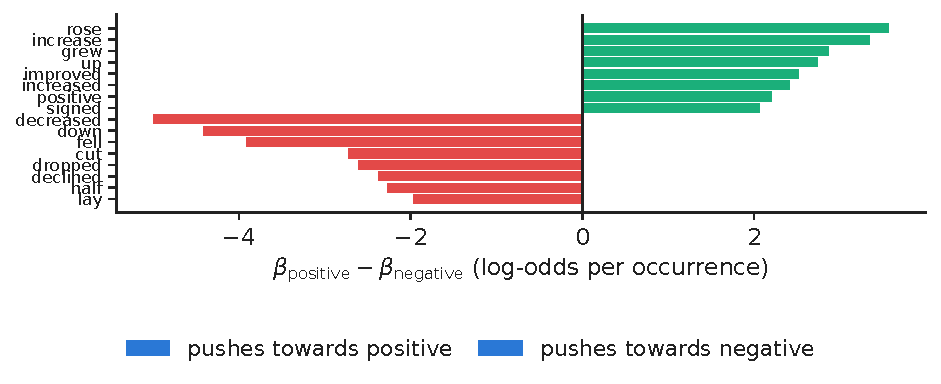
\includegraphics[width=\textwidth,height=0.312\textheight,keepaspectratio]{charts/en/top_words.pdf}\end{center}\vspace{-3mm}
\chartsource{Source: Financial PhraseBank (Malo et al., 2014). Data: 4,838 sentences of financial news, 5-8 annotators each.}
\vspace{0.5mm}
\begin{itemize}\setlength{\itemsep}{0pt}
  \item Most positive: rose, increase, grew, up, improved
    \begin{itemize}\setlength{\itemsep}{0pt}
      \item Most negative: decreased, down, fell, cut, dropped.
    \end{itemize}
  \item General-language dictionaries misread finance words (``liability'', ``tax''): learn the weights on finance text.
\end{itemize}
\par\vfill\noindent{\scriptsize\color{FooterGray}(Loughran \& McDonald, 2011; own computation)}\hfill\qlink{NN\_L6\_top\_words}{Quantlets/L6/NN_L6_top_words}\par\vspace{0.5mm}
\end{frame}


\section{Dense representations: word embeddings}

\begin{frame}{The distributional hypothesis}
\footnotesize
\intuition{words used in similar contexts get similar vectors; similarity is the cosine of the angle.}
\begin{columns}[T,onlytextwidth]
\begin{column}{0.53\textwidth}
\[ \mathbf e_w=\mathbf E^{\top}\mathbf o_w\in\R^{d},\qquad \cos(w,v)=\frac{\mathbf e_w^{\top}\mathbf e_v}{\|\mathbf e_w\|\,\|\mathbf e_v\|} \]{\footnotesize\begin{itemize}\setlength{\itemsep}{0pt}
  \item \textbf{\txtwhere}
    \begin{itemize}\setlength{\itemsep}{0pt}
      \item $\mathbf o_w\in\{0,1\}^{V}$ one-hot vector of word $w$
      \item $\mathbf E\in\R^{V\times d}$ embedding matrix, $d=100\ll V=8\,539$
      \item A lookup, not a product, in code
    \end{itemize}
\end{itemize}\par}
\end{column}
\begin{column}{0.44\textwidth}
\begin{itemize}\setlength{\itemsep}{2pt}
  \item One-hot vectors are orthogonal: ``inflation'' and ``prices'' have cosine 0.
  \item In our own embeddings: cos(inflation, prices) = 0.49, cos(inflation, climate) = 0.16, cos(banks, lending) = 0.46.
\end{itemize}
\end{column}
\end{columns}
\par\vfill\manager{dense vectors let a model trained on ``profit rose'' generalise to ``earnings increased''.}\par\vspace{0.5mm}
\par\vfill\noindent{\scriptsize\color{FooterGray}(Firth, 1957; Bishop \& Bishop, 2024, sec.~12.2)}\par\vspace{0.5mm}
\end{frame}

\begin{frame}{word2vec skip-gram: predict the context from the word}
\footnotesize
\intuition{each word in a window around the centre word is predicted by a softmax over the vocabulary.}
\begin{columns}[T,onlytextwidth]
\begin{column}{0.6\textwidth}
\[ \max_{\mathbf U,\mathbf V}\;\frac1T\sum_{t=1}^{T}\sum_{0<|j|\le c}\log p(w_{t+j}\mid w_t) \]\vspace{-2mm}\[ p(o\mid w)=\frac{\exp(\mathbf u_o^{\top}\mathbf v_w)}{\sum_{k=1}^{V}\exp(\mathbf u_k^{\top}\mathbf v_w)} \]{\footnotesize\begin{itemize}\setlength{\itemsep}{0pt}
  \item \textbf{\txtwhere}
    \begin{itemize}\setlength{\itemsep}{0pt}
      \item $\mathbf v_w$ input (centre) vector
      \item $\mathbf u_o$ output (context) vector
      \item $c$ window radius
      \item The denominator costs $O(V)$ per pair
    \end{itemize}
\end{itemize}\par}
\end{column}
\begin{column}{0.37\textwidth}
\begin{itemize}\setlength{\itemsep}{2pt}
  \item Continuous bag of words (CBOW) is the mirror image: predict the centre from the averaged context.
  \item The network is linear with one hidden layer
    \begin{itemize}\setlength{\itemsep}{0pt}
      \item The embeddings are its first weight matrix.
    \end{itemize}
  \item Our corpus: 3\,679\,754 (centre, context) pairs per epoch after subsampling.
\end{itemize}
\end{column}
\end{columns}
\par\vfill\manager{the full softmax over 8\,539 words is too slow
    \begin{itemize}\setlength{\itemsep}{0pt}
      \item Negative sampling replaces it.
    \end{itemize}}\par\vspace{0.5mm}
\par\vfill\noindent{\scriptsize\color{FooterGray}(Mikolov et al., 2013)}\par\vspace{0.5mm}
\end{frame}

\begin{frame}{Negative sampling: tell real pairs from random ones}
\footnotesize
\intuition{replace the softmax by $K+1$ binary logistic regressions: one real context word, $K$ noise words.}
\begin{columns}[T,onlytextwidth]
\begin{column}{0.53\textwidth}
\[ \ell(w,o)=-\log\sigma(\mathbf u_o^{\top}\mathbf v_w)-\sum_{k=1}^{K}\log\sigma(-\mathbf u_{n_k}^{\top}\mathbf v_w) \]\vspace{-2mm}\[ n_k\sim P_n(w)\propto f(w)^{3/4} \]{\footnotesize\begin{itemize}\setlength{\itemsep}{0pt}
  \item \textbf{\txtwhere}
    \begin{itemize}\setlength{\itemsep}{0pt}
      \item $\sigma$ logistic function
      \item $K=5$
      \item $f(w)$ corpus frequency
      \item Frequent words kept with probability $\min(1,\sqrt{t/f(w)}+t/f(w))$, $t=10^{-4}$
    \end{itemize}
\end{itemize}\par}
\end{column}
\begin{column}{0.44\textwidth}
\begin{itemize}\setlength{\itemsep}{2pt}
  \item Skip-gram with negative sampling (SGNS), $d=100$, window 5, words with at least 5 occurrences, Adam, 5 epochs in 120 seconds.
  \item Loss per pair from 2.622 (epoch 1) to 2.223.
  \item SGNS implicitly factorises a shifted pointwise mutual information (PMI) matrix (appendix).
\end{itemize}
\end{column}
\end{columns}
\par\vfill\manager{the same trick, contrast a true item with sampled negatives, trains recommender and fraud-embedding systems.}\par\vspace{0.5mm}
\par\vfill\noindent{\scriptsize\color{FooterGray}(Mikolov et al., 2013; Levy \& Goldberg, 2014)}\par\vspace{0.5mm}
\end{frame}

\begin{frame}{GloVe: fit the logarithm of the co-occurrence counts}
\footnotesize
\intuition{count once how often words appear together, then fit dot products to their logarithms with a weighted least-squares loss.}
\begin{columns}[T,onlytextwidth]
\begin{column}{0.5\textwidth}
\[ J=\sum_{i,j:\,X_{ij}>0}f(X_{ij})\big(\mathbf w_i^{\top}\tilde{\mathbf w}_j+b_i+\tilde b_j-\ln X_{ij}\big)^2 \]\vspace{-2mm}\[ f(x)=\min\{1,(x/x_{\max})^{\alpha}\} \]{\footnotesize\begin{itemize}\setlength{\itemsep}{0pt}
  \item \textbf{\txtwhere}
    \begin{itemize}\setlength{\itemsep}{0pt}
      \item $X_{ij}$ co-occurrences within 10 words, weighted $1/\text{distance}$
      \item $x_{\max}=100$, $\alpha=0.75$
      \item Final vector $\mathbf w_i+\tilde{\mathbf w}_i$
    \end{itemize}
\end{itemize}\par}
\end{column}
\begin{column}{0.47\textwidth}
\begin{center}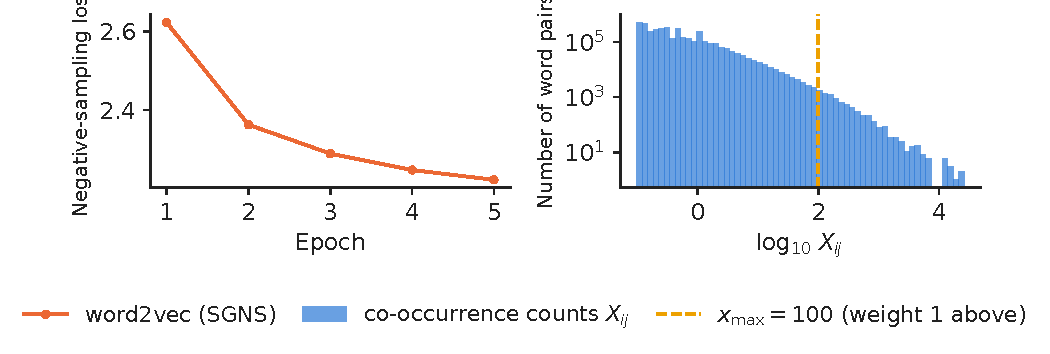
\includegraphics[width=\textwidth,height=0.500\textheight,keepaspectratio]{charts/en/emb_training.pdf}\end{center}\vspace{-3mm}
\chartsource{Source: European Central Bank, speeches dataset. Data: 8 Jan 2022 to 30 Oct 2026, 400 speeches.}
\end{column}
\end{columns}
\par\vfill\manager{3\,841\,517 non-zero pairs (5.269\,\% of $V^2$)
    \begin{itemize}\setlength{\itemsep}{0pt}
      \item 99.81\,\% are below $x_{\max}$ and get a weight below 1.
    \end{itemize}}\par\vspace{0.5mm}
\par\vfill\noindent{\scriptsize\color{FooterGray}(Pennington et al., 2014; own computation)}\hfill\qlink{NN\_L6\_emb\_training}{Quantlets/L6/NN_L6_emb_training}\par\vspace{0.5mm}
\end{frame}

\begin{frame}{Count-based word vectors: PMI and truncated matrix factorisation}
\footnotesize
\intuition{before neural embeddings, dense vectors came from factorising a matrix of word associations.}
\begin{columns}[T,onlytextwidth]
\begin{column}{0.6\textwidth}
\[ \mathrm{PMI}(w,c)=\ln\frac{P(w,c)}{P(w)P(c)} \]\vspace{-2mm}\[ \mathbf M_{+}\approx\mathbf U_d\boldsymbol\Sigma_d\mathbf V_d^{\top},\qquad \mathbf E=\mathbf U_d\boldsymbol\Sigma_d^{1/2} \]{\footnotesize\begin{itemize}\setlength{\itemsep}{0pt}
  \item \textbf{\txtwhere}
    \begin{itemize}\setlength{\itemsep}{0pt}
      \item $P(w,c)$ share of co-occurrences of $w$ and $c$
      \item $\mathbf M_{+}$ the matrix of $\max(\mathrm{PMI},0)$
      \item $\mathbf U_d,\boldsymbol\Sigma_d,\mathbf V_d$ the $d$ leading terms of the singular value decomposition (SVD)
    \end{itemize}
\end{itemize}\par}
\end{column}
\begin{column}{0.37\textwidth}
\begin{itemize}\setlength{\itemsep}{2pt}
  \item Pointwise mutual information (PMI) is positive when two words meet more often than chance.
  \item Our co-occurrence table has 3\,841\,517 non-zero pairs, 5.269\,\% of all $V^2$ cells: sparse, so the SVD is cheap.
  \item word2vec, GloVe and the SVD of PMI give similar neighbours on the same corpus.
\end{itemize}
\end{column}
\end{columns}
\par\vfill\manager{a factorisation of counts is transparent and reproducible: a good first embedding for an internal corpus.}\par\vspace{0.5mm}
\par\vfill\noindent{\scriptsize\color{FooterGray}(Levy \& Goldberg, 2014)}\par\vspace{0.5mm}
\end{frame}

\begin{frame}{Nearest neighbours in our central-bank embeddings}
\footnotesize
{\scriptsize\renewcommand{\arraystretch}{1.05}\setlength{\tabcolsep}{4pt}
\begin{tabular}{@{}p{0.13\textwidth}p{0.4\textwidth}p{0.4\textwidth}@{}}\toprule
Word & word2vec (SGNS) & GloVe \\ \midrule
\texttt{inflation} & headline, underlying, revert, hovering, medium & expectations, underlying, headline, core, term \\
\texttt{energy} & fertilisers, food, hicpxx, prices, renewable & prices, food, shock, commodity, renewable \\
\texttt{banks} & repaying, supervisors, themselves, obtaining, supervised & central, their, supervisors, they, have \\
\texttt{climate} & change, environmental, degradation, nature, ipcc & change, nature, environmental, related, risks \\
\texttt{digital} & convenient, functionality, kantar, erpb, payments & euro, payments, form, would, cash \\
\texttt{wages} & wage, profits, catch, negotiated, salaries & real, nominal, higher, incomes, rising \\
\texttt{ukraine} & invasion, russia, aggression, russian, brutal & invasion, russia, war, unjustified, russian \\
\texttt{rates} & interest, rate, compressed, hikes, repriced & interest, rate, short, lending, long \\
\bottomrule\end{tabular}}
\par\vspace{0.5mm}{\scriptsize \begin{itemize}\setlength{\itemsep}{0pt}
  \item Five nearest words by cosine; both trained on the same 1\,289\,896 tokens of ECB speeches; mean overlap of the two top-5 lists: 1.88 words.
\end{itemize}}
\par\vfill\manager{a central-bank watcher can expand a search for ``inflation'' with its learned neighbours instead of a hand-made list.}\par\vspace{0.5mm}
\par\vfill\noindent{\scriptsize\color{FooterGray}(own computation)}\hfill\tryit{\S2}\par\vspace{0.5mm}
\end{frame}

\begin{frame}{Topics of central banking form regions of the embedding space}
\small
\intuition{2-D principal component analysis (PCA) projection of 32 words chosen in four groups; the groups were not given to the model.}
\begin{center}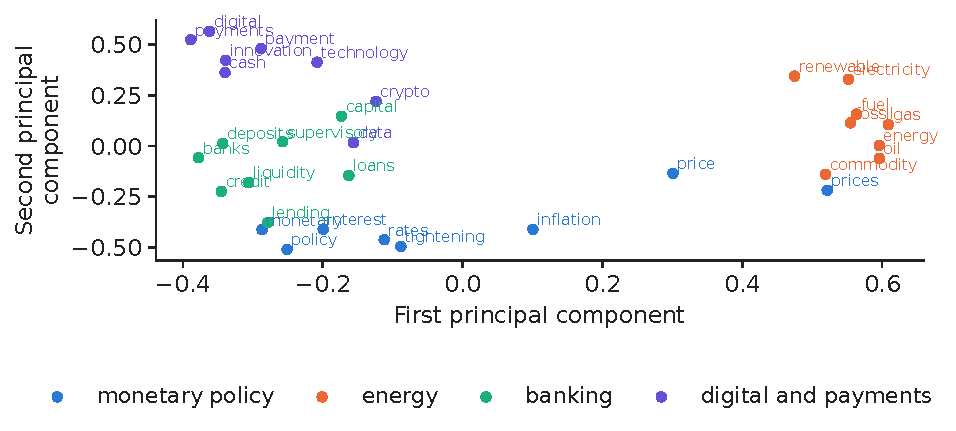
\includegraphics[width=\textwidth,height=0.500\textheight,keepaspectratio]{charts/en/w2v_pca.pdf}\end{center}\vspace{-3mm}
\chartsource{Source: European Central Bank, speeches dataset. Data: 8 Jan 2022 to 30 Oct 2026, 400 speeches.}
\vspace{0.5mm}
\begin{itemize}\setlength{\itemsep}{0pt}
  \item Two components keep 31.9\,\% of the variance of these 32 vectors, so the picture is a rough shadow of $\R^{100}$.
\end{itemize}
\par\vfill\noindent{\scriptsize\color{FooterGray}(own computation)}\hfill\qlink{NN\_L6\_w2v\_pca}{Quantlets/L6/NN_L6_w2v_pca}\par\vspace{0.5mm}
\end{frame}

\begin{frame}{Analogies, and the limits of one vector per word}
\footnotesize
\begin{columns}[T,onlytextwidth]
\begin{column}{0.46\textwidth}
{\scriptsize\renewcommand{\arraystretch}{1.05}\setlength{\tabcolsep}{4pt}
\begin{tabular}{@{}ll@{}}\toprule
$a:b::c:\,?$ & answer \\ \midrule
\texttt{germany : german : : france} & \texttt{fran} \\
\texttt{italy : italian : : spain} & \texttt{commissioned} \\
\texttt{banks : bank : : households} & \texttt{household} \\
\texttt{rise : rising : : fall} & \texttt{buffered} \\
\texttt{higher : lower : : increase} & \texttt{marginal} \\
\bottomrule\end{tabular}}
\par\vspace{0.5mm}{\scriptsize \begin{itemize}\setlength{\itemsep}{0pt}
  \item Answer $=\argmax_v\cos(\mathbf e_v,\mathbf e_b-\mathbf e_a+\mathbf e_c)$, excluding $a,b,c$; our word2vec, one small corpus.
\end{itemize}}
\end{column}
\begin{column}{0.51\textwidth}
\begin{itemize}\setlength{\itemsep}{4pt}
  \item \textbf{Static embeddings}
    \begin{itemize}\setlength{\itemsep}{0pt}
      \item One vector per word type, whatever the sentence
      \item ``interest'' (rate) and ``interest'' (attention) share a vector; so do ``bank'' and ``bank''
    \end{itemize}
  \item \textbf{Coverage}
    \begin{itemize}\setlength{\itemsep}{0pt}
      \item The ECB vocabulary covers 84.7\,\% of PhraseBank tokens and 76.4\,\% of tweet tokens
      \item The rest are out of vocabulary (OOV); subword models (fastText) and transformers (Lecture 7) address both problems
    \end{itemize}
\end{itemize}
\end{column}
\end{columns}
\par\vfill\noindent{\scriptsize\color{FooterGray}(Mikolov et al., 2013; Bojanowski et al., 2017)}\par\vspace{0.5mm}
\end{frame}

\begin{frame}{Subword vectors for words never seen}
\footnotesize
\intuition{build a word vector from the vectors of its character $n$-grams, so a new ticker or a typo still gets a vector.}
\begin{columns}[T,onlytextwidth]
\begin{column}{0.53\textwidth}
\[ \mathbf e_w=\sum_{g\in\mathcal G(w)}\mathbf z_g \]{\footnotesize\begin{itemize}\setlength{\itemsep}{0pt}
  \item \textbf{\txtwhere}
    \begin{itemize}\setlength{\itemsep}{0pt}
      \item $\mathcal G(w)$ the character $n$-grams of $w$ (for example 3 to 6 characters, with boundary symbols) and the word itself
      \item $\mathbf z_g$ learned $n$-gram vectors
    \end{itemize}
\end{itemize}\par}
\end{column}
\begin{column}{0.44\textwidth}
\begin{itemize}\setlength{\itemsep}{2pt}
  \item Coverage of our word-level ECB vocabulary: 84.7\,\% of PhraseBank tokens, 76.4\,\% of tweet tokens.
  \item Subword models (fastText) share information between ``profit'', ``profits'' and ``profitability''.
  \item Transformers (Lecture 7) use the same idea with learned subword tokens.
\end{itemize}
\end{column}
\end{columns}
\par\vfill\manager{for tweets and chat messages, with tickers and spelling variants, use subword vectors or a subword tokeniser.}\par\vspace{0.5mm}
\par\vfill\noindent{\scriptsize\color{FooterGray}(Bojanowski et al., 2017)}\par\vspace{0.5mm}
\end{frame}


\section{Sentence classifiers: sparse versus dense}

\begin{frame}{An embedding-bag network: average the word vectors, then a softmax}
\footnotesize
\intuition{the simplest neural text classifier learns the embeddings and the classifier together.}
\begin{columns}[T,onlytextwidth]
\begin{column}{0.53\textwidth}
\[ \mathbf z=\frac{1}{|S|}\sum_{s\in S}\mathbf e_s \]\vspace{-2mm}\[ \hat{\mathbf p}=\softmax(\mW\,\mathrm{dropout}(\mathbf z)+\vb) \]\vspace{-2mm}\[ \loss=-\frac1n\sum_i\omega_{y_i}\log\hat p_{i,y_i} \]{\footnotesize\begin{itemize}\setlength{\itemsep}{0pt}
  \item \textbf{\txtwhere}
    \begin{itemize}\setlength{\itemsep}{0pt}
      \item $S$ the tokens and bigrams of the sentence
      \item $\mathbf e_s$ learned vectors ($d=100$)
      \item $\omega_k=n/(3n_k)$ class weights against the dominance of ``neutral''
    \end{itemize}
\end{itemize}\par}
\end{column}
\begin{column}{0.44\textwidth}
\begin{itemize}\setlength{\itemsep}{2pt}
  \item Random start, or word2vec start: rows of $\mathbf E$ initialised with our ECB vectors, then fine-tuned.
  \item Also compared: mean word2vec vector + logistic regression (frozen), TF-IDF + a multilayer perceptron (MLP) with 128 hidden units.
\end{itemize}
\end{column}
\end{columns}
\par\vfill\manager{this is the architecture of fastText-type classifiers, used in production for millions of documents per hour.}\par\vspace{0.5mm}
\par\vfill\noindent{\scriptsize\color{FooterGray}(Joulin et al., 2017)}\par\vspace{0.5mm}
\end{frame}

\begin{frame}{Logistic regression on text: the gradient}
\footnotesize
\intuition{the multinomial logistic model is a one-layer network; its gradient compares predicted and true class shares.}
\begin{columns}[T,onlytextwidth]
\begin{column}{0.53\textwidth}
\[ \loss(\mathbf B)=-\sum_{i}\sum_k y_{ik}\ln\hat p_{ik}+\frac{1}{2C}\|\mathbf B\|_F^2 \]\vspace{-2mm}\[ \nabla_{\mathbf B}\loss=\mathbf X^{\top}(\hat{\mathbf P}-\mathbf Y)+\mathbf B/C \]{\footnotesize\begin{itemize}\setlength{\itemsep}{0pt}
  \item \textbf{\txtwhere}
    \begin{itemize}\setlength{\itemsep}{0pt}
      \item $\mathbf X$ the TF-IDF matrix ($n\times V$, sparse)
      \item $\mathbf Y$ one-hot labels
      \item $\hat{\mathbf P}$ softmax probabilities
      \item $C$ inverse penalty, chosen on validation from $\{0.1,1,10\}$
    \end{itemize}
\end{itemize}\par}
\end{column}
\begin{column}{0.44\textwidth}
\begin{itemize}\setlength{\itemsep}{2pt}
  \item Convex loss: one optimum, no seed to report
    \begin{itemize}\setlength{\itemsep}{0pt}
      \item The multilayer perceptron (MLP) on the same inputs adds a hidden layer of 128 units.
    \end{itemize}
  \item PhraseBank macro-F1: logistic 73.49\,\%, MLP 71.37\,\%: the hidden layer does not help here.
\end{itemize}
\end{column}
\end{columns}
\par\vfill\manager{with a few thousand short sentences, the extra flexibility of a network buys variance, not accuracy.}\par\vspace{0.5mm}
\par\vfill\noindent{\scriptsize\color{FooterGray}(own computation)}\par\vspace{0.5mm}
\end{frame}

\begin{frame}{From word vectors to a sentence vector}
\footnotesize
\intuition{averaging word vectors is the simplest sentence representation, and it loses what matters for sentiment.}
\begin{columns}[T,onlytextwidth]
\begin{column}{0.53\textwidth}
\[ \mathbf s_i=\frac{1}{|S_i|}\sum_{w\in S_i}\mathbf e_w,\qquad \mathbf s_i^{\mathrm{w}}=\frac{\sum_{w}a_w\mathbf e_w}{\sum_w a_w},\ \ a_w=\frac{\alpha}{\alpha+f(w)} \]{\footnotesize\begin{itemize}\setlength{\itemsep}{0pt}
  \item \textbf{\txtwhere}
    \begin{itemize}\setlength{\itemsep}{0pt}
      \item $S_i$ the in-vocabulary tokens of sentence $i$
      \item $a_w$ a weight that down-weights frequent words
      \item $\alpha$ a small constant
    \end{itemize}
\end{itemize}\par}
\end{column}
\begin{column}{0.44\textwidth}
\begin{itemize}\setlength{\itemsep}{2pt}
  \item Mean of our frozen ECB vectors + logistic regression: macro-F1 57.30\,\% on PhraseBank, 53.71\,\% on tweets.
  \item ``rose'' and ``fell'' are close in a co-occurrence space (same contexts), so the average blurs the sign.
  \item Fine-tuning the vectors on labelled data (embedding bag) recovers most of the gap.
\end{itemize}
\end{column}
\end{columns}
\par\vfill\manager{generic embeddings are good for search and similarity, not automatically for sentiment.}\par\vspace{0.5mm}
\par\vfill\noindent{\scriptsize\color{FooterGray}(own computation)}\par\vspace{0.5mm}
\end{frame}

\begin{frame}{Protocol and metric: macro-F1 on an imbalanced target}
\footnotesize
\intuition{``neutral'' is 59.3\,\% of PhraseBank, so accuracy rewards a model that says ``neutral'' all the time.}
\begin{columns}[T,onlytextwidth]
\begin{column}{0.53\textwidth}
\[ \mathrm{F1}_k=\frac{2P_kR_k}{P_k+R_k},\qquad \text{macro-F1}=\frac13\sum_{k=1}^{3}\mathrm{F1}_k \]{\footnotesize\begin{itemize}\setlength{\itemsep}{0pt}
  \item \textbf{\txtwhere}
    \begin{itemize}\setlength{\itemsep}{0pt}
      \item $P_k$ precision and $R_k$ recall of class $k$
      \item Each class counts equally, whatever its size
    \end{itemize}
\end{itemize}\par}
\end{column}
\begin{column}{0.44\textwidth}
\begin{itemize}\setlength{\itemsep}{2pt}
  \item PhraseBank: 5 random stratified splits 70/15/15
    \begin{itemize}\setlength{\itemsep}{0pt}
      \item Tweets: published validation split used as test, 3 seeds.
    \end{itemize}
  \item Penalty $C$, early stopping and vocabulary are chosen on the validation part only.
\end{itemize}
\end{column}
\end{columns}
\par\vfill\manager{for an alert system, report the recall of the negative class next to the macro-F1: that is the class that costs money.}\par\vspace{0.5mm}
\par\vfill\noindent{\scriptsize\color{FooterGray}(own computation)}\hfill\tryit{\S3}\par\vspace{0.5mm}
\end{frame}

\begin{frame}{On short financial sentences, TF-IDF is hard to beat}
\small
\intuition{test macro-F1 of seven representations and classifiers, PhraseBank and finance tweets (bars: mean, whiskers: standard deviation).}
\begin{center}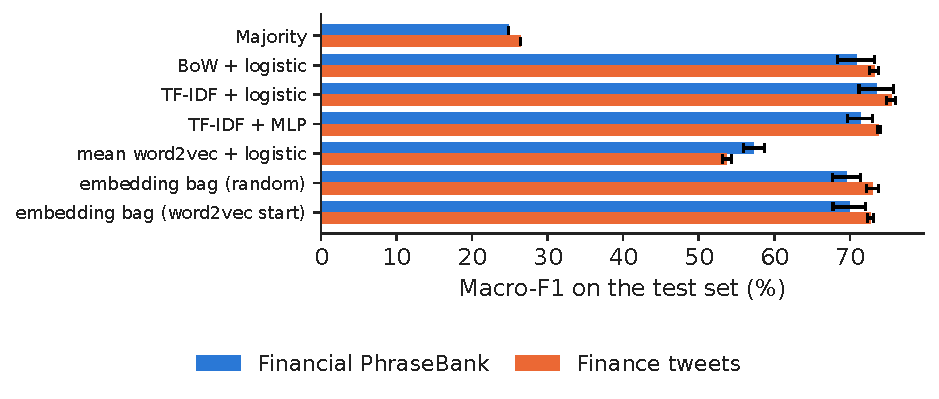
\includegraphics[width=\textwidth,height=0.470\textheight,keepaspectratio]{charts/en/sentiment_models.pdf}\end{center}\vspace{-3mm}
\chartsource{Source: Financial PhraseBank (Malo et al., 2014); Twitter financial news (Hugging Face, zeroshot). Data: PhraseBank: 5 random 70/15/15 splits; tweets: published validation split as test, 3 seeds.}
\vspace{0.5mm}
\begin{itemize}\setlength{\itemsep}{0pt}
  \item Best on PhraseBank: 73.49 (TF-IDF + logistic) vs 69.93 (embedding bag, word2vec start)
    \begin{itemize}\setlength{\itemsep}{0pt}
      \item Majority 24.81.
    \end{itemize}
\end{itemize}
\par\vfill\noindent{\scriptsize\color{FooterGray}(own computation)}\hfill\qlink{NN\_L6\_sentiment\_models}{Quantlets/L6/NN_L6_sentiment_models}\par\vspace{0.5mm}
\end{frame}

\begin{frame}{Sentiment results, with uncertainty}
\footnotesize
{\scriptsize\renewcommand{\arraystretch}{1.05}\setlength{\tabcolsep}{4pt}
\begin{tabular}{@{}lrrrr@{}}\toprule
Model & PhraseBank macro-F1 & acc. & Tweets macro-F1 & acc. \\ \midrule
Majority class & 24.81\,$\pm$\,0.00 & 59.28 & 26.40\,$\pm$\,0.00 & 65.58 \\
BoW + logistic & 70.82\,$\pm$\,2.41 & 74.94 & 73.25\,$\pm$\,0.59 & 80.00 \\
TF-IDF + logistic & 73.49\,$\pm$\,2.28 & 77.69 & 75.47\,$\pm$\,0.56 & 81.77 \\
TF-IDF + MLP & 71.37\,$\pm$\,1.65 & 76.23 & 73.85\,$\pm$\,0.24 & 80.56 \\
mean word2vec + logistic & 57.30\,$\pm$\,1.39 & 62.01 & 53.71\,$\pm$\,0.60 & 61.59 \\
embedding bag, random start & 69.56\,$\pm$\,1.81 & 74.11 & 72.97\,$\pm$\,0.78 & 79.77 \\
embedding bag, word2vec start & 69.93\,$\pm$\,2.16 & 74.99 & 72.76\,$\pm$\,0.39 & 79.51 \\
\bottomrule\end{tabular}}
\par\vspace{0.5mm}{\scriptsize \begin{itemize}\setlength{\itemsep}{0pt}
  \item Paired over the 5 PhraseBank splits: TF-IDF + logistic minus embedding bag (word2vec start) $=\ensuremath{+}3.55$ points, $t=9.88$ (4 degrees of freedom).
  \item Starting from our ECB word2vec vectors changes the embedding bag by \ensuremath{+}0.37 points on PhraseBank and \ensuremath{-}0.21 on tweets.
\end{itemize}}
\par\vfill\manager{the cheapest model within one standard deviation of the best is the one to deploy and explain.}\par\vspace{0.5mm}
\par\vfill\noindent{\scriptsize\color{FooterGray}(own computation)}\par\vspace{0.5mm}
\end{frame}

\begin{frame}{How large should the embedding be?}
\footnotesize
\begin{columns}[T,onlytextwidth]
\begin{column}{0.35\textwidth}
{\footnotesize\renewcommand{\arraystretch}{1.05}\setlength{\tabcolsep}{4pt}
\begin{tabular}{@{}rr@{}}\toprule
Dimension $d$ & Macro-F1 (\%) \\ \midrule
8 & 67.3 \\
16 & 66.5 \\
32 & 67.2 \\
64 & 67.8 \\
128 & 68.8 \\
256 & 67.3 \\
\bottomrule\end{tabular}}
\par\vspace{0.5mm}{\scriptsize \begin{itemize}\setlength{\itemsep}{0pt}
  \item Embedding bag, random start, PhraseBank split 1, mean of 3 seeds.
\end{itemize}}
\end{column}
\begin{column}{0.62\textwidth}
\begin{itemize}\setlength{\itemsep}{4pt}
  \item Parameters of the embedding layer: $V\times d$
    \begin{itemize}\setlength{\itemsep}{0pt}
      \item With bigrams $V$ is several thousand, so $d$ drives the model size.
    \end{itemize}
  \item Here the score is flat in $d$: from 67.3 at $d=8$ to 68.8 at $d=128$.
  \item A three-class task on short sentences needs few dimensions
    \begin{itemize}\setlength{\itemsep}{0pt}
      \item General-purpose embeddings use 100--300 because they serve many tasks.
    \end{itemize}
\end{itemize}
\end{column}
\end{columns}
\par\vfill\manager{choose $d$ on validation data
    \begin{itemize}\setlength{\itemsep}{0pt}
      \item A smaller model is cheaper to serve and to explain.
    \end{itemize}}\par\vspace{0.5mm}
\par\vfill\noindent{\scriptsize\color{FooterGray}(own computation)}\par\vspace{0.5mm}
\end{frame}

\begin{frame}{Classification errors and annotator agreement}
\small
\intuition{test accuracy by the share of annotators who agreed on the label of the sentence.}
\begin{center}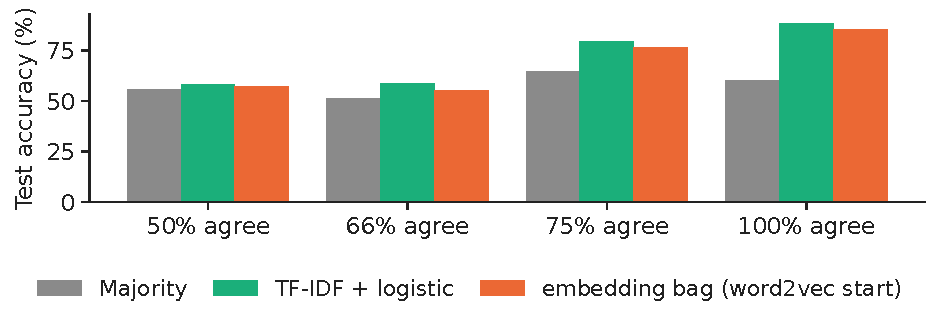
\includegraphics[width=\textwidth,height=0.420\textheight,keepaspectratio]{charts/en/agreement.pdf}\end{center}\vspace{-3mm}
\chartsource{Source: Financial PhraseBank (Malo et al., 2014). Data: test sentences of 5 random splits, by share of annotators that agree.}
\vspace{0.5mm}
\begin{itemize}\setlength{\itemsep}{0pt}
  \item TF-IDF + logistic: 88.4\,\% on unanimous sentences, 58.1\,\% on 50\,\% agreement
    \begin{itemize}\setlength{\itemsep}{0pt}
      \item 2\,259 of 4\,838 sentences are unanimous.
    \end{itemize}
\end{itemize}
\par\vfill\manager{label noise caps every model: before buying a bigger model, check how much your own analysts agree.}\par\vspace{0.5mm}
\par\vfill\noindent{\scriptsize\color{FooterGray}(own computation)}\hfill\qlink{NN\_L6\_agreement}{Quantlets/L6/NN_L6_agreement}\par\vspace{0.5mm}
\end{frame}

\begin{frame}{With few labels, a word2vec start helps the network; TF-IDF stays competitive}
\small
\intuition{left: test macro-F1 against the number of labelled sentences; right: embedding size of the embedding bag.}
\begin{center}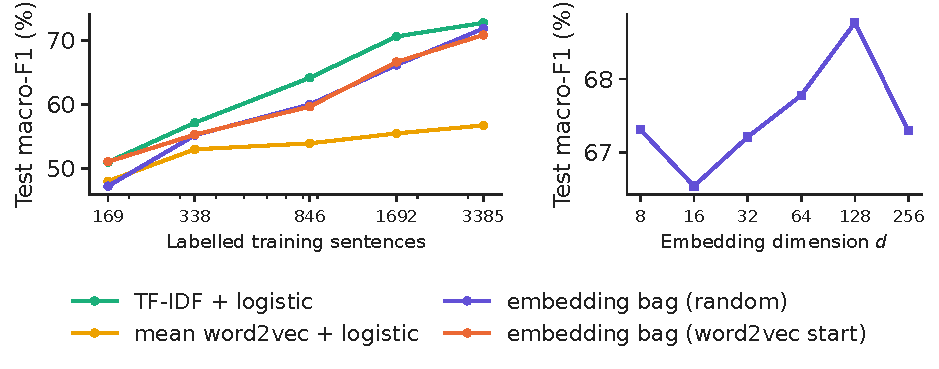
\includegraphics[width=\textwidth,height=0.420\textheight,keepaspectratio]{charts/en/learning_curve.pdf}\end{center}\vspace{-3mm}
\chartsource{Source: Financial PhraseBank (Malo et al., 2014). Data: left: 3 random splits; right: embedding bag (random start), split 1, 3 seeds.}
\vspace{0.5mm}
\begin{itemize}\setlength{\itemsep}{0pt}
  \item With 169 labelled sentences: TF-IDF 51.0, mean word2vec 48.0, embedding bag random 47.2, word2vec start 51.0
    \begin{itemize}\setlength{\itemsep}{0pt}
      \item With all 3\,385: 72.8, 56.7, 71.9, 70.9.
    \end{itemize}
\end{itemize}
\par\vfill\noindent{\scriptsize\color{FooterGray}(own computation)}\hfill\qlink{NN\_L6\_learning\_curve}{Quantlets/L6/NN_L6_learning_curve}\par\vspace{0.5mm}
\end{frame}

\begin{frame}{Where the errors are: negative news read as neutral}
\footnotesize
\begin{columns}[T,onlytextwidth]
\begin{column}{0.47\textwidth}
{\footnotesize\renewcommand{\arraystretch}{1.05}\setlength{\tabcolsep}{4pt}
\begin{tabular}{@{}lrrr@{}}\toprule
True \textbackslash{} predicted & neg. & neu. & pos. \\ \midrule
negative & -- & 107 & 48 \\
positive & 50 & 263 & -- \\
\bottomrule\end{tabular}}
\par\vspace{0.5mm}{\scriptsize \begin{itemize}\setlength{\itemsep}{0pt}
  \item TF-IDF + logistic, the 5 PhraseBank test sets pooled (3\,635 sentences).
\end{itemize}}
\end{column}
\begin{column}{0.5\textwidth}
\begin{itemize}\setlength{\itemsep}{4pt}
  \item Recall: negative 65.9\,\%, neutral 84.1\,\%, positive 69.5\,\%.
  \item Opposite-sign errors are rare
    \begin{itemize}\setlength{\itemsep}{0pt}
      \item Most errors move a sentence to neutral.
    \end{itemize}
  \item Typical miss: a fall described with neutral words and numbers (``sales were EUR 10 mn, down from 12'').
\end{itemize}
\end{column}
\end{columns}
\par\vfill\manager{numbers carry sentiment in finance
    \begin{itemize}\setlength{\itemsep}{0pt}
      \item Mapping them all to one token loses ``down from''-type comparisons that a sequence model can read.
    \end{itemize}}\par\vspace{0.5mm}
\par\vfill\noindent{\scriptsize\color{FooterGray}(own computation)}\par\vspace{0.5mm}
\end{frame}


\section{Case study: topics of finance tweets}

\begin{frame}{Twenty topics: easy for earnings and the Fed, hard for general news}
\small
\intuition{per-topic F1 on the 4\,117 test tweets (published validation split).}
\begin{center}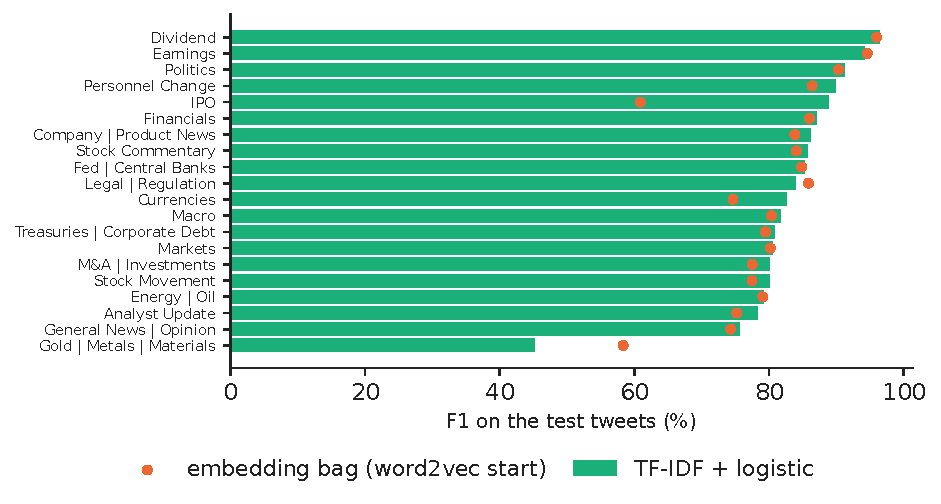
\includegraphics[width=\textwidth,height=0.550\textheight,keepaspectratio]{charts/en/topic_f1.pdf}\end{center}\vspace{-3mm}
\chartsource{Source: Twitter financial news datasets (Hugging Face, zeroshot). Data: 4,117 test tweets (published validation split), 20 topics.}
\vspace{0.5mm}
\begin{itemize}\setlength{\itemsep}{0pt}
  \item Macro-F1: TF-IDF + logistic 82.62\,\%, embedding bag (word2vec start) 80.45\,\%
    \begin{itemize}\setlength{\itemsep}{0pt}
      \item Accuracy 84.48\,\% vs 20.69\,\% for the majority topic.
    \end{itemize}
\end{itemize}
\par\vfill\noindent{\scriptsize\color{FooterGray}(own computation)}\hfill\qlink{NN\_L6\_topic\_f1}{Quantlets/L6/NN_L6_topic_f1}\par\vspace{0.5mm}
\end{frame}

\begin{frame}{Text models at work in finance}
\footnotesize
\begin{columns}[T,onlytextwidth]
\begin{column}{0.5\textwidth}
\begin{itemize}\setlength{\itemsep}{3pt}
  \item \textbf{News and tweet triage}
    \begin{itemize}\setlength{\itemsep}{0pt}
      \item Route items by topic (best: Dividend, F1 96.4\,\%) and flag negative ones for the analyst
    \end{itemize}
  \item \textbf{Central-bank communication}
    \begin{itemize}\setlength{\itemsep}{0pt}
      \item Track words near ``inflation'' or ``energy'' speech by speech
    \end{itemize}
  \item \textbf{Compliance and environmental, social and governance (ESG) screening}
    \begin{itemize}\setlength{\itemsep}{0pt}
      \item Search reports with learned synonyms, not fixed keyword lists
    \end{itemize}
\end{itemize}
\end{column}
\begin{column}{0.47\textwidth}
\begin{itemize}\setlength{\itemsep}{3pt}
  \item \textbf{Limits of today's models}
    \begin{itemize}\setlength{\itemsep}{0pt}
      \item Word order beyond bigrams is lost
      \item One vector per word ignores context
      \item Weakest topic: Gold | Metals | Materials, F1 45.2\,\%
    \end{itemize}
  \item \textbf{Next: attention}
    \begin{itemize}\setlength{\itemsep}{0pt}
      \item Contextual vectors from transformers, e.g. bidirectional encoder representations from transformers (BERT) and a BERT model adapted to financial text (FinBERT), in Lecture 7, compared fairly with these baselines
    \end{itemize}
\end{itemize}
\end{column}
\end{columns}
\par\vfill\manager{start every text project with TF-IDF + logistic regression
    \begin{itemize}\setlength{\itemsep}{0pt}
      \item Move to embeddings or transformers only when the gain is shown on your data.
    \end{itemize}}\par\vspace{0.5mm}
\par\vfill\noindent{\scriptsize\color{FooterGray}(own computation)}\par\vspace{0.5mm}
\end{frame}

\section*{Wrap-up}

\begin{frame}{Quiz 1: idf}
\small
\begin{itemize}
  \item A word appears in every one of the $n$ training sentences
    \begin{itemize}\setlength{\itemsep}{0pt}
      \item What is its smoothed idf?
    \end{itemize}
\end{itemize}
\vspace{2mm}
\begin{exampleblock}{Answer}
\begin{itemize}
  \item $\ln\frac{1+n}{1+n}+1=1$: the minimum, so it barely moves the normalised vector.
\end{itemize}
\end{exampleblock}
\end{frame}

\begin{frame}{Quiz 2: negative sampling}
\small
\begin{itemize}
  \item Why does word2vec draw negative words from $f(w)^{3/4}$ and not from $f(w)$?
\end{itemize}
\vspace{2mm}
\begin{exampleblock}{Answer}
\begin{itemize}
  \item The power 3/4 flattens the distribution: rare words are drawn more often than their frequency, frequent ones like ``the'' less, which gives more useful contrasts.
\end{itemize}
\end{exampleblock}
\end{frame}

\begin{frame}{Quiz 3: accuracy}
\small
\begin{itemize}
  \item A vendor reports 60\,\% accuracy on PhraseBank sentiment
    \begin{itemize}\setlength{\itemsep}{0pt}
      \item Is it good?
    \end{itemize}
\end{itemize}
\vspace{2mm}
\begin{exampleblock}{Answer}
\begin{itemize}
  \item No: always ``neutral'' gives 59.28\,\%
    \begin{itemize}\setlength{\itemsep}{0pt}
      \item Ask for macro-F1 (our TF-IDF + logistic: 73.49\,\%).
    \end{itemize}
\end{itemize}
\end{exampleblock}
\end{frame}

\begin{frame}{Quiz 4: transfer}
\small
\begin{itemize}
  \item You have only 169 labelled sentences
    \begin{itemize}\setlength{\itemsep}{0pt}
      \item Which representation helps most?
    \end{itemize}
\end{itemize}
\vspace{2mm}
\begin{exampleblock}{Answer}
\begin{itemize}
  \item Compare on validation data: here mean word2vec gives 48.0, TF-IDF 51.0, embedding bag with word2vec start 51.0 macro-F1.
\end{itemize}
\end{exampleblock}
\end{frame}

\begin{frame}{Quiz 5: polysemy}
\small
\begin{itemize}
  \item Why can a static embedding not separate ``interest rate'' from ``of interest to investors''?
\end{itemize}
\vspace{2mm}
\begin{exampleblock}{Answer}
\begin{itemize}
  \item It has one vector per word type, the average of all its uses
    \begin{itemize}\setlength{\itemsep}{0pt}
      \item Contextual models (Lecture 7) give a different vector in each sentence.
    \end{itemize}
\end{itemize}
\end{exampleblock}
\end{frame}

\begin{frame}{Wrap-up}
\small
\vspace{-2mm}\begin{multicols}{2}\scriptsize\tableofcontents\end{multicols}
\begin{itemize}\setlength{\itemsep}{1pt}
  \item Text becomes numbers through tokens and counts (BoW, TF-IDF) or dense vectors (word2vec, GloVe) learned from co-occurrence.
  \item On real financial sentences TF-IDF + logistic regression is the model to beat
    \begin{itemize}\setlength{\itemsep}{0pt}
      \item A word2vec start helps the network only when labels are few.
      \item Next: attention and transformers (Lecture 7).
    \end{itemize}
\end{itemize}
\end{frame}

\begin{frame}{Research from our group: language models for finance}
\footnotesize
\begin{itemize}\setlength{\itemsep}{4pt}
  \item \textbf{Large language models (LLM) forecast value-at-risk (VaR) and expected shortfall (ES)} (Pele, Bolovăneanu, Lin, Ren, Ginavar, Spilak, Andrei, Toma, Lessmann \& Härdle, 2026, Expert Systems with Applications)
    \begin{itemize}\setlength{\itemsep}{0pt}
      \item Paper: ``In the beginning was the Word: LLM-VaR and LLM-ES''; LLM forecasts benchmarked against classical risk models with formal backtests
      \item Text models move from sentiment scores to the risk numbers themselves (Lecture 12)
    \end{itemize}
  \item \textbf{BitMood: artificial intelligence (AI) analysis of Bitcoin trends via Facebook emotions} (Conda, Găman, Bâg, Mazurencu-Marinescu-Pele, Pele \& Härdle, 2026, Digital Finance)
    \begin{itemize}\setlength{\itemsep}{0pt}
      \item 120,000 Facebook posts, 2015--2023, classified with FinBERT into compound sentiment scores with the reactions of readers
      \item Sentiment predicts Bitcoin trading volume; sentiment-based strategies outperform buy-and-hold; topic modelling tracks the themes of the discussion
    \end{itemize}
\end{itemize}
\par\vspace{0.5mm}{\scriptsize \begin{itemize}\setlength{\itemsep}{0pt}
  \item Findings as stated in the papers; numbers on the other slides come from our own computations.
\end{itemize}}
\par\vfill\noindent{\scriptsize\color{FooterGray}(Bucharest University of Economic Studies; Romanian Academy, Institute for Economic Forecasting)}\par\vspace{0.5mm}
\end{frame}

\begin{frame}{Want to learn more?}
\small
\begin{columns}[T,onlytextwidth]
\begin{column}{0.52\textwidth}
\begin{itemize}\setlength{\itemsep}{4pt}
  \item \textbf{Mikolov et al. (2013)} and \textbf{Pennington et al. (2014)}: the two embedding papers, both short.
  \item \textbf{Levy \& Goldberg (2014)}: why word2vec is a matrix factorisation.
  \item \textbf{Loughran \& McDonald (2011)}: the finance sentiment dictionary and why general dictionaries fail.
\end{itemize}
\end{column}
\begin{column}{0.45\textwidth}
\begin{itemize}\setlength{\itemsep}{4pt}
  \item \textbf{This course}: code, data, notebooks --- \href{https://github.com/danpele/NEURAL_BIZ}{github.com/danpele/NEURAL\_BIZ}.
  \item \textbf{Experiment yourself}: the notebook reproduces the charts of this lecture --- \href{\nnrepo/\nnnb}{notebooks/}.
  \item \textbf{Seminar 6}: a sentiment index of ECB speeches built with your own classifier.
\end{itemize}
\end{column}
\end{columns}
\end{frame}

\begin{frame}{References (1/2)}
\scriptsize
\begin{itemize}\setlength{\itemsep}{0pt}\scriptsize
\item Bishop, C.\,M.\ \& Bishop, H.\ (2024). \textit{Deep Learning: Foundations and Concepts}, ch.~12. Springer. \href{https://doi.org/10.1007/978-3-031-45468-4}{doi:10.1007/978-3-031-45468-4}
\item Bojanowski, P., Grave, E., Joulin, A.\ \& Mikolov, T.\ (2017). Enriching word vectors with subword information. \textit{TACL}, 5, 135--146. \href{https://doi.org/10.1162/tacl_a_00051}{doi:10.1162/tacl\_a\_00051}
\item Conda, A.\,I., Găman, Ș., Bâg, R.\,C., Mazurencu-Marinescu-Pele, M., Pele, D.\,T.\ \& Härdle, W.\,K.\ (2026). BitMood: AI analysis of Bitcoin trends via Facebook emotions. \textit{Digital Finance}, 8(3), 42. \href{https://doi.org/10.1007/s42521-026-00205-3}{doi:10.1007/s42521-026-00205-3}
\item Firth, J.\,R.\ (1957). A synopsis of linguistic theory 1930--1955. In \textit{Studies in Linguistic Analysis}, 1--32. Blackwell.
\item Joulin, A., Grave, E., Bojanowski, P.\ \& Mikolov, T.\ (2017). Bag of tricks for efficient text classification. \textit{EACL}, 427--431. \href{https://doi.org/10.18653/v1/E17-2068}{doi:10.18653/v1/E17-2068}
\item Levy, O.\ \& Goldberg, Y.\ (2014). Neural word embedding as implicit matrix factorization. \textit{NIPS}, 27, 2177--2185. \href{https://papers.nips.cc/paper/5477-neural-word-embedding-as-implicit-matrix-factorization}{papers.nips.cc}
\item Loughran, T.\ \& McDonald, B.\ (2011). When is a liability not a liability? Textual analysis, dictionaries, and 10-Ks. \textit{Journal of Finance}, 66(1), 35--65. \href{https://doi.org/10.1111/j.1540-6261.2010.01625.x}{doi:10.1111/j.1540-6261.2010.01625.x}
\end{itemize}
\end{frame}

\begin{frame}{References (2/2)}
\scriptsize
\begin{itemize}\setlength{\itemsep}{0pt}\scriptsize
\item Malo, P., Sinha, A., Korhonen, P., Wallenius, J.\ \& Takala, P.\ (2014). Good debt or bad debt: Detecting semantic orientations in economic texts. \textit{JASIST}, 65(4), 782--796. \href{https://doi.org/10.1002/asi.23062}{doi:10.1002/asi.23062}
\item Mikolov, T., Sutskever, I., Chen, K., Corrado, G.\ \& Dean, J.\ (2013). Distributed representations of words and phrases and their compositionality. \textit{NIPS}, 26, 3111--3119. \href{https://arxiv.org/abs/1310.4546}{arXiv:1310.4546}
\item Pele, D.\,T., Bolovăneanu, V., Lin, M.-B., Ren, R., Ginavar, A.\,T., Spilak, B., Andrei, A.-V., Toma, F.-M., Lessmann, S.\ \& Härdle, W.\,K.\ (2026). In the beginning was the Word: LLM-VaR and LLM-ES. \textit{Expert Systems with Applications}, 295, 128676. \href{https://doi.org/10.1016/j.eswa.2025.128676}{doi:10.1016/j.eswa.2025.128676}
\item Pennington, J., Socher, R.\ \& Manning, C.\,D.\ (2014). GloVe: Global vectors for word representation. \textit{EMNLP}, 1532--1543. \href{https://doi.org/10.3115/v1/D14-1162}{doi:10.3115/v1/D14-1162}
\item Salton, G.\ \& Buckley, C.\ (1988). Term-weighting approaches in automatic text retrieval. \textit{Information Processing \& Management}, 24(5), 513--523. \href{https://doi.org/10.1016/0306-4573(88)90021-0}{doi:10.1016/0306-4573(88)90021-0}
\item Zipf, G.\,K.\ (1949). \textit{Human Behavior and the Principle of Least Effort}. Addison-Wesley.
\end{itemize}
\end{frame}

\appendix

\begin{frame}{Appendix: the gradient of negative sampling}
\footnotesize
\begin{itemize}\setlength{\itemsep}{3pt}
  \item For one pair, $\ell=-\log\sigma(s_o)-\sum_k\log\sigma(-s_k)$ with $s_o=\mathbf u_o^{\top}\mathbf v_w$, $s_k=\mathbf u_{n_k}^{\top}\mathbf v_w$.
  \item Using $\frac{d}{ds}\log\sigma(s)=1-\sigma(s)$: $\partial\ell/\partial\mathbf v_w=-(1-\sigma(s_o))\mathbf u_o+\sum_k\sigma(s_k)\mathbf u_{n_k}$.
  \item $\partial\ell/\partial\mathbf u_o=-(1-\sigma(s_o))\mathbf v_w$ and $\partial\ell/\partial\mathbf u_{n_k}=\sigma(s_k)\mathbf v_w$: real contexts are pulled closer, noise words pushed away.
  \item At the optimum, $\mathbf u_o^{\top}\mathbf v_w=\mathrm{PMI}(w,o)-\ln K$, with $\mathrm{PMI}(w,o)=\ln\frac{P(w,o)}{P(w)P(o)}$ (Levy \& Goldberg, 2014).
\end{itemize}
\end{frame}

\begin{frame}{Appendix: the models in code}
\footnotesize
{\scriptsize\ttfamily\setlength{\parindent}{0pt}tf = TfidfVectorizer(ngram\_range=(1, 2), min\_df=2, sublinear\_tf=True).fit(train\_text)\\
clf = LogisticRegression(C=C, class\_weight='balanced', max\_iter=3000).fit(tf.transform(train\_text), y)\\
\mbox{}\\
class EmbBag(nn.Module):\ \ \ \ \ \ \ \ \ \ \ \ \ \ \ \ \ \ \ \ \ \ \ \  \# fastText-style classifier\\
\hspace*{2.0em}def \_\_init\_\_(self, n\_vocab, dim, n\_cls):\\
\hspace*{4.0em}super().\_\_init\_\_()\\
\hspace*{4.0em}self.emb = nn.EmbeddingBag(n\_vocab, dim, mode='mean')\\
\hspace*{4.0em}self.out = nn.Linear(dim, n\_cls)\\
\hspace*{2.0em}def forward(self, ids, offsets):\\
\hspace*{4.0em}return self.out(F.dropout(self.emb(ids, offsets), 0.3, self.training))\\
\# SGNS step: loss = -(logsigmoid((v*u\_pos).sum(1)) + logsigmoid(-(U\_neg @ v[...,None]).squeeze()).sum(1)).mean()\par}\begin{itemize}\setlength{\itemsep}{2pt}
  \item Full code: lectures/L6/analysis\_L6.py and the notebook of this lecture.
\end{itemize}
\end{frame}

\end{document}
